\documentclass[letterpaper]{book}
\usepackage{makeidx}
\usepackage{natbib}
\usepackage{graphicx}
\usepackage{multicol}
\usepackage{float}
\usepackage{listings}
\usepackage{color}
\usepackage{ifthen}
\usepackage[table]{xcolor}
\usepackage{textcomp}
\usepackage{alltt}
\usepackage{ifpdf}
\ifpdf
\usepackage[pdftex,
            pagebackref=true,
            colorlinks=true,
            linkcolor=blue,
            unicode
           ]{hyperref}
\else
\usepackage[ps2pdf,
            pagebackref=true,
            colorlinks=true,
            linkcolor=blue,
            unicode
           ]{hyperref}
\usepackage{pspicture}
\fi
\usepackage[utf8]{inputenc}
\usepackage{mathptmx}
\usepackage[scaled=.90]{helvet}
\usepackage{courier}
\usepackage{sectsty}
\usepackage[titles]{tocloft}
\usepackage{doxygen}
\lstset{language=C++,inputencoding=utf8,basicstyle=\footnotesize,breaklines=true,breakatwhitespace=true,tabsize=4,numbers=left }
\makeindex
\setcounter{tocdepth}{3}
\renewcommand{\footrulewidth}{0.4pt}
\renewcommand{\familydefault}{\sfdefault}
\hfuzz=15pt
\setlength{\emergencystretch}{15pt}
\hbadness=750
\tolerance=750
\begin{document}
\hypersetup{pageanchor=false,citecolor=blue}
\begin{titlepage}
\vspace*{7cm}
\begin{center}
{\Large \-Inter-\/task communication tests \\[1ex]\large 0.\-4 }\\
\vspace*{1cm}
{\large \-Generated by Doxygen 1.7.6.1}\\
\vspace*{0.5cm}
{\small Mon Apr 21 2014 15:22:35}\\
\end{center}
\end{titlepage}
\clearemptydoublepage
\pagenumbering{roman}
\tableofcontents
\clearemptydoublepage
\pagenumbering{arabic}
\hypersetup{pageanchor=true,citecolor=blue}
\chapter{\-Inter-\/task communication tests}
\label{index}\hypertarget{index}{}This program implements a set of tests to verify that the M\+E405 library's inter-\/task communication works. It's also a usable example of how the queues and shared data items are used. In addition, it helps to show why non thread safe data transfer is a bad idea; there is a global variable used to pass data between two tasks, and as the program runs, the global variable sometimes gets corrupted.

The task diagram for this program is shown below. \begin{center}

\begin{DoxyImageNoCaption}
  \mbox{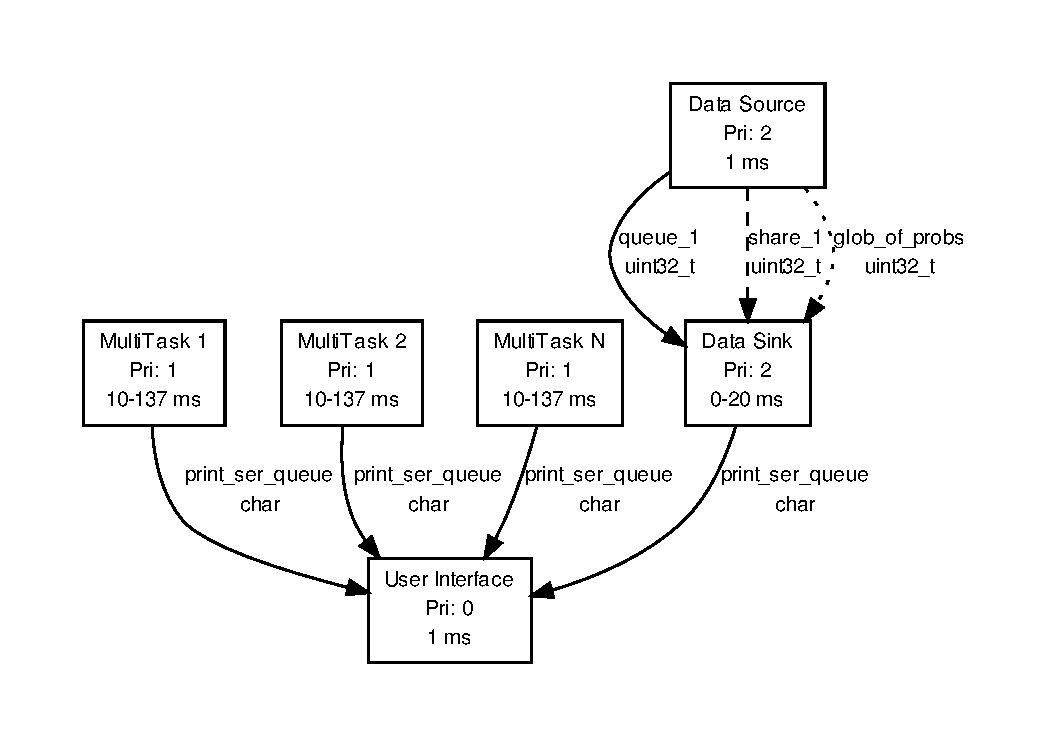
\includegraphics[width=\textwidth,height=\textheight/2,keepaspectratio=true]{dot_inline_dotgraph_1}}
\end{DoxyImageNoCaption}
\end{center}
 There are a couple of unusual features on this task diagram. The number of \char`\"{}multi-\/tasks\char`\"{} can be varied by changing {\ttfamily N\+\_\+\+M\+U\+L\+T\+I\+\_\+\+T\+A\+S\+K\+S} in {\ttfamily \hyperlink{test__main_8cpp_a840291bc02cba5474a4cb46a9b9566fe}{main()}}. These multi-\/tasks are a bunch of tasks, all created from the same class, that are used to put some stress on the R\+T\+O\+S by running lots of tasks at the same time. The multi-\/task's timing includes a delay of random duration; this timing scheme causes tasks to pre-\/empt each other with random timing. The data sink task normally runs very quickly, looking for changed data; if it finds data, it delays by 20 ms to give other tasks some time to run. The data sink therefore takes up a lot of C\+P\+U time, and one can see that the user interface runs slowly because of this.

When this program is running, one can press the \char`\"{}v\char`\"{} key in a terminal window to cause the program to display a task status report. A typical report is shown below. 
\begin{DoxyCode}
Task                            Stack
Name            Pri.    State   Free/Total      Runs
----            ----    -----   ----------      ----
Multi3          1       0       63/120          0        153 runs
Multi2          1       0       63/120          0        161 runs
Multi1          1       0       63/120          0        157 runs
Multi0          1       0       63/120          0        152 runs
UserInt         1       0       66/240          0        4217 runs
Sink            2       0       92/160          0       1136446 runs, errors in queue: 0, shared\_data: 0, 
      global data: 265
Source          2       0       145/220         0        10446 runs
IDLE            0       -       50/100
Heap: 4000/5944, OCR5A=1999
\end{DoxyCode}
 This report shows tasks and their current priorities and states. Also, for the data sink task, it shows a report of how accurately the data from the data source task has been received. One should see that there have been no errors in sending data through the queue or shared data item, but the use of a global variable has caused errors due to task switching while the data was being written or read. 
\chapter{\-Class \-Index}
\section{\-Class \-List}
\-Here are the classes, structs, unions and interfaces with brief descriptions\-:\begin{DoxyCompactList}
\item\contentsline{section}{\hyperlink{classadc}{adc} \\*\-This class should run the \-A/\-D converter on an \-A\-V\-R processor }{\pageref{classadc}}{}
\item\contentsline{section}{\hyperlink{classmotor__driver}{motor\-\_\-driver} \\*\-This class runs the motor on the h-\/bridge chip }{\pageref{classmotor__driver}}{}
\item\contentsline{section}{\hyperlink{classtask__motor}{task\-\_\-motor} }{\pageref{classtask__motor}}{}
\item\contentsline{section}{\hyperlink{classtask__multi}{task\-\_\-multi} }{\pageref{classtask__multi}}{}
\item\contentsline{section}{\hyperlink{classtask__sink}{task\-\_\-sink} }{\pageref{classtask__sink}}{}
\item\contentsline{section}{\hyperlink{classtask__source}{task\-\_\-source} }{\pageref{classtask__source}}{}
\item\contentsline{section}{\hyperlink{classtask__user}{task\-\_\-user} }{\pageref{classtask__user}}{}
\end{DoxyCompactList}

\chapter{\-File \-Index}
\section{File List}
Here is a list of all documented files with brief descriptions\+:\begin{DoxyCompactList}
\item\contentsline{section}{\hyperlink{adc_8cpp}{adc.\+cpp} }{\pageref{adc_8cpp}}{}
\item\contentsline{section}{\hyperlink{adc_8h}{adc.\+h} }{\pageref{adc_8h}}{}
\item\contentsline{section}{\hyperlink{motor__driver_8cpp}{motor\+\_\+driver.\+cpp} }{\pageref{motor__driver_8cpp}}{}
\item\contentsline{section}{\hyperlink{motor__driver_8h}{motor\+\_\+driver.\+h} }{\pageref{motor__driver_8h}}{}
\item\contentsline{section}{\hyperlink{shares_8h}{shares.\+h} }{\pageref{shares_8h}}{}
\item\contentsline{section}{{\bfseries task\+\_\+motor.\+cpp} }{\pageref{task__motor_8cpp}}{}
\item\contentsline{section}{{\bfseries task\+\_\+motor.\+h} }{\pageref{task__motor_8h}}{}
\item\contentsline{section}{\hyperlink{task__user_8cpp}{task\+\_\+user.\+cpp} }{\pageref{task__user_8cpp}}{}
\item\contentsline{section}{\hyperlink{task__user_8h}{task\+\_\+user.\+h} }{\pageref{task__user_8h}}{}
\item\contentsline{section}{\hyperlink{test__main_8cpp}{test\+\_\+main.\+cpp} }{\pageref{test__main_8cpp}}{}
\end{DoxyCompactList}

\chapter{\-Class \-Documentation}
\hypertarget{classadc}{\section{adc \-Class \-Reference}
\label{classadc}\index{adc@{adc}}
}


\-This class should run the \-A/\-D converter on an \-A\-V\-R processor.  




{\ttfamily \#include $<$adc.\-h$>$}

\subsection*{\-Public \-Member \-Functions}
\begin{DoxyCompactItemize}
\item 
\hyperlink{classadc_af3b8262c08f5fc5ae325a20622883424}{adc} (emstream $\ast$=\-N\-U\-L\-L)
\begin{DoxyCompactList}\small\item\em \-This constructor sets up an \-A/\-D converter. \end{DoxyCompactList}\item 
uint16\-\_\-t \hyperlink{classadc_a2190a59696a7093e1ea605e998ccf97e}{read\-\_\-once} (uint8\-\_\-t)
\begin{DoxyCompactList}\small\item\em \-This method takes one \-A/\-D reading from the given channel and returns it. \end{DoxyCompactList}\item 
uint16\-\_\-t \hyperlink{classadc_a58f1030fe64d3dea4ccd8a2687dd6fce}{read\-\_\-oversampled} (uint8\-\_\-t, uint8\-\_\-t)
\begin{DoxyCompactList}\small\item\em \-This method finds the average result while guarding against overflow. \end{DoxyCompactList}\end{DoxyCompactItemize}
\subsection*{\-Protected \-Attributes}
\begin{DoxyCompactItemize}
\item 
\hypertarget{classadc_a14680b48b723bf1adddd2741ebb18a3e}{emstream $\ast$ \hyperlink{classadc_a14680b48b723bf1adddd2741ebb18a3e}{ptr\-\_\-to\-\_\-serial}}\label{classadc_a14680b48b723bf1adddd2741ebb18a3e}

\begin{DoxyCompactList}\small\item\em \-The \-A\-D\-C class uses this pointer to the serial port to say hello. \end{DoxyCompactList}\item 
\hypertarget{classadc_a6df75e4965d01b573c088c052e9c80c6}{uint8\-\_\-t \hyperlink{classadc_a6df75e4965d01b573c088c052e9c80c6}{\-A\-D\-M\-U\-X\-\_\-init}}\label{classadc_a6df75e4965d01b573c088c052e9c80c6}

\begin{DoxyCompactList}\small\item\em \-Initial admux value. \end{DoxyCompactList}\end{DoxyCompactItemize}


\subsection{\-Detailed \-Description}
\-This class should run the \-A/\-D converter on an \-A\-V\-R processor. 

\-It should have some better comments. \-Yes, this is a {\bfseries subtle} {\bfseries hint}. 

\-Definition at line 45 of file adc.\-h.



\subsection{\-Constructor \& \-Destructor \-Documentation}
\hypertarget{classadc_af3b8262c08f5fc5ae325a20622883424}{\index{adc@{adc}!adc@{adc}}
\index{adc@{adc}!adc@{adc}}
\subsubsection[{adc}]{\setlength{\rightskip}{0pt plus 5cm}{\bf adc\-::adc} (
\begin{DoxyParamCaption}
\item[{emstream $\ast$}]{p\-\_\-serial\-\_\-port = {\ttfamily \-N\-U\-L\-L}}
\end{DoxyParamCaption}
)}}\label{classadc_af3b8262c08f5fc5ae325a20622883424}


\-This constructor sets up an \-A/\-D converter. 

{\bfseries \-Details\-:} \-The \-A/\-D converter is enabled and the division factor is set to 32. 
\begin{DoxyParams}{\-Parameters}
{\em p\-\_\-serial\-\_\-port} & \-A pointer to the serial port where debugging info is written. \\
\hline
\end{DoxyParams}


\-Definition at line 42 of file adc.\-cpp.



\-References \-A\-D\-M\-U\-X\-\_\-init, and ptr\-\_\-to\-\_\-serial.



\subsection{\-Member \-Function \-Documentation}
\hypertarget{classadc_a2190a59696a7093e1ea605e998ccf97e}{\index{adc@{adc}!read\-\_\-once@{read\-\_\-once}}
\index{read\-\_\-once@{read\-\_\-once}!adc@{adc}}
\subsubsection[{read\-\_\-once}]{\setlength{\rightskip}{0pt plus 5cm}uint16\-\_\-t {\bf adc\-::read\-\_\-once} (
\begin{DoxyParamCaption}
\item[{uint8\-\_\-t}]{ch}
\end{DoxyParamCaption}
)}}\label{classadc_a2190a59696a7093e1ea605e998ccf97e}


\-This method takes one \-A/\-D reading from the given channel and returns it. 

{\bfseries \-Details\-:} \-This method selects a channel to read and goes through the \-A/\-D conversion. \-This method also guards against time-\/out. 
\begin{DoxyParams}{\-Parameters}
{\em ch} & \-The \-A/\-D channel which is being read must be from 0 to 7. \\
\hline
\end{DoxyParams}
\begin{DoxyReturn}{\-Returns}
\-The result of the \-A/\-D conversion. 
\end{DoxyReturn}


\-Definition at line 65 of file adc.\-cpp.



\-References \-A\-D\-M\-U\-X\-\_\-init.



\-Referenced by read\-\_\-oversampled(), and task\-\_\-motor\-::run().

\hypertarget{classadc_a58f1030fe64d3dea4ccd8a2687dd6fce}{\index{adc@{adc}!read\-\_\-oversampled@{read\-\_\-oversampled}}
\index{read\-\_\-oversampled@{read\-\_\-oversampled}!adc@{adc}}
\subsubsection[{read\-\_\-oversampled}]{\setlength{\rightskip}{0pt plus 5cm}uint16\-\_\-t {\bf adc\-::read\-\_\-oversampled} (
\begin{DoxyParamCaption}
\item[{uint8\-\_\-t}]{channel, }
\item[{uint8\-\_\-t}]{samples}
\end{DoxyParamCaption}
)}}\label{classadc_a58f1030fe64d3dea4ccd8a2687dd6fce}


\-This method finds the average result while guarding against overflow. 

{\bfseries \-Details\-:} \-This method first checks to see whether the number of samples will threaten overflow and then saturates the number of samples if necessary. \-It then takes the average. 
\begin{DoxyParams}{\-Parameters}
{\em channel} & \-A selected channel to read from. \\
\hline
{\em samples} & \-The chosen number of samples. \\
\hline
\end{DoxyParams}
\begin{DoxyReturn}{\-Returns}
\-The average readings from a chosen number of samples. 
\end{DoxyReturn}


\-Definition at line 94 of file adc.\-cpp.



\-References read\-\_\-once().



\-The documentation for this class was generated from the following files\-:\begin{DoxyCompactItemize}
\item 
\hyperlink{adc_8h}{adc.\-h}\item 
\hyperlink{adc_8cpp}{adc.\-cpp}\end{DoxyCompactItemize}

\hypertarget{classmotor__driver}{\section{motor\-\_\-driver \-Class \-Reference}
\label{classmotor__driver}\index{motor\-\_\-driver@{motor\-\_\-driver}}
}


\-This class runs the motor on the h-\/bridge chip.  




{\ttfamily \#include $<$motor\-\_\-driver.\-h$>$}

\subsection*{\-Public \-Member \-Functions}
\begin{DoxyCompactItemize}
\item 
\hyperlink{classmotor__driver_a8ae335815e1a1ef23904750562639346}{motor\-\_\-driver} (emstream $\ast$p\-\_\-serial\-\_\-port, volatile uint8\-\_\-t $\ast$p\-\_\-ddr, uint8\-\_\-t ddr\-\_\-mask, volatile uint8\-\_\-t $\ast$pwm, uint8\-\_\-t pwm\-\_\-mask, volatile uint8\-\_\-t $\ast$p\-\_\-port, uint8\-\_\-t enable\-\_\-mask, volatile uint8\-\_\-t $\ast$p\-\_\-tccra, uint8\-\_\-t tccra\-\_\-mask, volatile uint8\-\_\-t $\ast$p\-\_\-tccrb, uint8\-\_\-t tccrb\-\_\-mask, volatile uint16\-\_\-t $\ast$p\-\_\-ocr)
\begin{DoxyCompactList}\small\item\em \-This constructor sets up a motor driver. \end{DoxyCompactList}\item 
void \hyperlink{classmotor__driver_ae8f7bd6aa553abf071abcebc876a9e10}{set\-\_\-power} (int16\-\_\-t power)
\begin{DoxyCompactList}\small\item\em \-This method sets direction and duty cycle of the motor. \end{DoxyCompactList}\item 
void \hyperlink{classmotor__driver_aa21e7894053cd83968d9e6b2958c9aec}{brake} (void)
\begin{DoxyCompactList}\small\item\em \-This method stops the motor. \end{DoxyCompactList}\end{DoxyCompactItemize}
\subsection*{\-Protected \-Attributes}
\begin{DoxyCompactItemize}
\item 
\hypertarget{classmotor__driver_a5d94686caee87309fc36257bcab1035f}{emstream $\ast$ \hyperlink{classmotor__driver_a5d94686caee87309fc36257bcab1035f}{ptr\-\_\-to\-\_\-serial}}\label{classmotor__driver_a5d94686caee87309fc36257bcab1035f}

\begin{DoxyCompactList}\small\item\em \-The motor driver class uses this pointer print to the serial port. \end{DoxyCompactList}\item 
\hypertarget{classmotor__driver_a3c15d9a1839e286d7f5081b471c6f967}{volatile uint16\-\_\-t $\ast$ \hyperlink{classmotor__driver_a3c15d9a1839e286d7f5081b471c6f967}{compare}}\label{classmotor__driver_a3c15d9a1839e286d7f5081b471c6f967}

\begin{DoxyCompactList}\small\item\em \-This points to the compare register. \end{DoxyCompactList}\item 
\hypertarget{classmotor__driver_a0a51fcc2cd6c747fa6e892c3b00cf575}{volatile uint8\-\_\-t $\ast$ \hyperlink{classmotor__driver_a0a51fcc2cd6c747fa6e892c3b00cf575}{direction}}\label{classmotor__driver_a0a51fcc2cd6c747fa6e892c3b00cf575}

\begin{DoxyCompactList}\small\item\em \-This points to the direction register. \end{DoxyCompactList}\item 
\hypertarget{classmotor__driver_a3679745ec176df2d78ce091cd2a55589}{uint8\-\_\-t \hyperlink{classmotor__driver_a3679745ec176df2d78ce091cd2a55589}{enable}}\label{classmotor__driver_a3679745ec176df2d78ce091cd2a55589}

\begin{DoxyCompactList}\small\item\em \-Enable pin on h-\/bridge chip. \end{DoxyCompactList}\end{DoxyCompactItemize}


\subsection{\-Detailed \-Description}
\-This class runs the motor on the h-\/bridge chip. 

\-This class takes in several ports and their inputs and masks for a specific motherboard, as well as a serial port. 

\-Definition at line 26 of file motor\-\_\-driver.\-h.



\subsection{\-Constructor \& \-Destructor \-Documentation}
\hypertarget{classmotor__driver_a8ae335815e1a1ef23904750562639346}{\index{motor\-\_\-driver@{motor\-\_\-driver}!motor\-\_\-driver@{motor\-\_\-driver}}
\index{motor\-\_\-driver@{motor\-\_\-driver}!motor_driver@{motor\-\_\-driver}}
\subsubsection[{motor\-\_\-driver}]{\setlength{\rightskip}{0pt plus 5cm}{\bf motor\-\_\-driver\-::motor\-\_\-driver} (
\begin{DoxyParamCaption}
\item[{emstream $\ast$}]{p\-\_\-serial\-\_\-port, }
\item[{volatile uint8\-\_\-t $\ast$}]{p\-\_\-ddr, }
\item[{uint8\-\_\-t}]{ddr\-\_\-mask, }
\item[{volatile uint8\-\_\-t $\ast$}]{p\-\_\-pwm, }
\item[{uint8\-\_\-t}]{pwm\-\_\-mask, }
\item[{volatile uint8\-\_\-t $\ast$}]{p\-\_\-port, }
\item[{uint8\-\_\-t}]{enable\-\_\-mask, }
\item[{volatile uint8\-\_\-t $\ast$}]{p\-\_\-tccra, }
\item[{uint8\-\_\-t}]{tccra\-\_\-mask, }
\item[{volatile uint8\-\_\-t $\ast$}]{p\-\_\-tccrb, }
\item[{uint8\-\_\-t}]{tccrb\-\_\-mask, }
\item[{volatile uint16\-\_\-t $\ast$}]{p\-\_\-ocr}
\end{DoxyParamCaption}
)}}\label{classmotor__driver_a8ae335815e1a1ef23904750562639346}


\-This constructor sets up a motor driver. 

{\bfseries \-Details\-:} \-The motor driver is enabled based on parameters. \-The motor initial spins clockwise. 
\begin{DoxyParams}{\-Parameters}
{\em p\-\_\-serial\-\_\-port} & \-A pointer to the serial port where debugging info is written. \\
\hline
{\em p\-\_\-ddr} & \-A pointer to the \-D\-D\-Rx for \-I\-Nx and \-D\-I\-A\-Gx on h-\/bridge chip. \\
\hline
{\em ddr\-\_\-mask} & \-Enable pin settings on h-\/bridge chip. \\
\hline
{\em p\-\_\-pwm} & \-A pointer to the \-D\-D\-Rx for pwn pin on h-\/bridge chip. \\
\hline
{\em pwm\-\_\-mask} & \-Enable pwm pin on h-\/bridge chip. \\
\hline
{\em p\-\_\-port} & \-A pointer to enable h-\/bridge chip. \\
\hline
{\em enable\-\_\-mask} & \-A mask for the \-D\-I\-A\-G/\-E\-N pin for h-\/bridge chip. \\
\hline
{\em p\-\_\-tccra} & \-A pointer to the timer/counter register \-A. \\
\hline
{\em tccra\-\_\-mask} & \-Timer/counter register \-A mask. \\
\hline
{\em p\-\_\-tccrb} & \-A pointer to the timer/counter register \-B. \\
\hline
{\em tccrb\-\_\-mask} & \-Timer/counter register \-B mask. \\
\hline
{\em p\-\_\-ocr} & \-A pointer to the output compare register. \\
\hline
\end{DoxyParams}


\-Definition at line 34 of file motor\-\_\-driver.\-cpp.



\-References compare, direction, enable, and ptr\-\_\-to\-\_\-serial.



\subsection{\-Member \-Function \-Documentation}
\hypertarget{classmotor__driver_aa21e7894053cd83968d9e6b2958c9aec}{\index{motor\-\_\-driver@{motor\-\_\-driver}!brake@{brake}}
\index{brake@{brake}!motor_driver@{motor\-\_\-driver}}
\subsubsection[{brake}]{\setlength{\rightskip}{0pt plus 5cm}void {\bf motor\-\_\-driver\-::brake} (
\begin{DoxyParamCaption}
\item[{void}]{}
\end{DoxyParamCaption}
)}}\label{classmotor__driver_aa21e7894053cd83968d9e6b2958c9aec}


\-This method stops the motor. 

{\bfseries \-Details\-:} \-This method brakes the motor to ground. 

\-Definition at line 86 of file motor\-\_\-driver.\-cpp.



\-References direction, and enable.



\-Referenced by task\-\_\-motor\-::run().

\hypertarget{classmotor__driver_ae8f7bd6aa553abf071abcebc876a9e10}{\index{motor\-\_\-driver@{motor\-\_\-driver}!set\-\_\-power@{set\-\_\-power}}
\index{set\-\_\-power@{set\-\_\-power}!motor_driver@{motor\-\_\-driver}}
\subsubsection[{set\-\_\-power}]{\setlength{\rightskip}{0pt plus 5cm}void {\bf motor\-\_\-driver\-::set\-\_\-power} (
\begin{DoxyParamCaption}
\item[{int16\-\_\-t}]{power}
\end{DoxyParamCaption}
)}}\label{classmotor__driver_ae8f7bd6aa553abf071abcebc876a9e10}


\-This method sets direction and duty cycle of the motor. 

{\bfseries \-Details\-:} \-This method determines direction and sets the duty cycle. 
\begin{DoxyParams}{\-Parameters}
{\em power} & power setting, negative number reverse motor direction \mbox{[}-\/255, 255\mbox{]}. \\
\hline
\end{DoxyParams}


\-Definition at line 69 of file motor\-\_\-driver.\-cpp.



\-References compare, direction, and enable.



\-Referenced by task\-\_\-motor\-::run().



\-The documentation for this class was generated from the following files\-:\begin{DoxyCompactItemize}
\item 
\hyperlink{motor__driver_8h}{motor\-\_\-driver.\-h}\item 
\hyperlink{motor__driver_8cpp}{motor\-\_\-driver.\-cpp}\end{DoxyCompactItemize}

\hypertarget{classtask__motor}{\section{task\-\_\-motor \-Class \-Reference}
\label{classtask__motor}\index{task\-\_\-motor@{task\-\_\-motor}}
}


{\ttfamily \#include $<$task\-\_\-motor.\-h$>$}

\subsection*{\-Public \-Member \-Functions}
\begin{DoxyCompactItemize}
\item 
\hyperlink{classtask__motor_a94cd580f333660de457fdc5c2bd5702e}{task\-\_\-motor} (const char $\ast$, unsigned port\-B\-A\-S\-E\-\_\-\-T\-Y\-P\-E, size\-\_\-t, uint8\-\_\-t, \hyperlink{classmotor__driver}{motor\-\_\-driver} $\ast$, shared\-\_\-data$<$ bool $>$ $\ast$, shared\-\_\-data$<$ int16\-\_\-t $>$ $\ast$, shared\-\_\-data$<$ bool $>$ $\ast$, uint8\-\_\-t, emstream $\ast$)
\item 
void \hyperlink{classtask__motor_a895a075ec470c9d5a07b8959de06aacd}{run} (void)
\item 
void \hyperlink{classtask__motor_ae855a78d1ee432a797d401a9222c9955}{print\-\_\-status} (emstream \&)
\end{DoxyCompactItemize}
\subsection*{\-Public \-Attributes}
\begin{DoxyCompactItemize}
\item 
\hypertarget{classtask__motor_a54a068b1d4cb46dba17d3de8d17fc87c}{uint32\-\_\-t \hyperlink{classtask__motor_a54a068b1d4cb46dba17d3de8d17fc87c}{runs}}\label{classtask__motor_a54a068b1d4cb46dba17d3de8d17fc87c}

\begin{DoxyCompactList}\small\item\em \-How many times through the task loop. \end{DoxyCompactList}\end{DoxyCompactItemize}
\subsection*{\-Protected \-Attributes}
\begin{DoxyCompactItemize}
\item 
\hypertarget{classtask__motor_a3f10bbf8d028b18a2a4427f1c152be53}{uint8\-\_\-t \hyperlink{classtask__motor_a3f10bbf8d028b18a2a4427f1c152be53}{brake\-\_\-pin}}\label{classtask__motor_a3f10bbf8d028b18a2a4427f1c152be53}

\begin{DoxyCompactList}\small\item\em \-Brake pin mask. \end{DoxyCompactList}\item 
\hypertarget{classtask__motor_ae64744376a44ba347c8f37afd7311ab7}{uint8\-\_\-t \hyperlink{classtask__motor_ae64744376a44ba347c8f37afd7311ab7}{adc\-\_\-select}}\label{classtask__motor_ae64744376a44ba347c8f37afd7311ab7}

\begin{DoxyCompactList}\small\item\em \-Value for which adc should read from. \end{DoxyCompactList}\item 
\hypertarget{classtask__motor_ad9d344255e29de67611998bf77658d9f}{\hyperlink{classmotor__driver}{motor\-\_\-driver} $\ast$ \hyperlink{classtask__motor_ad9d344255e29de67611998bf77658d9f}{driver}}\label{classtask__motor_ad9d344255e29de67611998bf77658d9f}

\begin{DoxyCompactList}\small\item\em \-A pointer to \hyperlink{classmotor__driver}{motor\-\_\-driver}. \end{DoxyCompactList}\item 
\hypertarget{classtask__motor_a22d847bf1b45ed005a6f6393cb37d327}{shared\-\_\-data$<$ bool $>$ $\ast$ \hyperlink{classtask__motor_a22d847bf1b45ed005a6f6393cb37d327}{brake}}\label{classtask__motor_a22d847bf1b45ed005a6f6393cb37d327}

\begin{DoxyCompactList}\small\item\em \-A pointer to the brake shared data. \end{DoxyCompactList}\item 
\hypertarget{classtask__motor_a291245b7c83dae649f310caf016ab959}{shared\-\_\-data$<$ int16\-\_\-t $>$ $\ast$ \hyperlink{classtask__motor_a291245b7c83dae649f310caf016ab959}{power}}\label{classtask__motor_a291245b7c83dae649f310caf016ab959}

\begin{DoxyCompactList}\small\item\em \-A pointer to the power shared data. \end{DoxyCompactList}\item 
\hypertarget{classtask__motor_afe8cab4e912b4814d29a8b9f0d091f48}{shared\-\_\-data$<$ bool $>$ $\ast$ \hyperlink{classtask__motor_afe8cab4e912b4814d29a8b9f0d091f48}{pot}}\label{classtask__motor_afe8cab4e912b4814d29a8b9f0d091f48}

\begin{DoxyCompactList}\small\item\em \-A pointer to the potentiometer shared data. \end{DoxyCompactList}\end{DoxyCompactItemize}


\subsection{\-Detailed \-Description}
\-This task determines what commands to send to the motor driver. 

\-Definition at line 32 of file task\-\_\-motor.\-h.



\subsection{\-Constructor \& \-Destructor \-Documentation}
\hypertarget{classtask__motor_a94cd580f333660de457fdc5c2bd5702e}{\index{task\-\_\-motor@{task\-\_\-motor}!task\-\_\-motor@{task\-\_\-motor}}
\index{task\-\_\-motor@{task\-\_\-motor}!task_motor@{task\-\_\-motor}}
\subsubsection[{task\-\_\-motor}]{\setlength{\rightskip}{0pt plus 5cm}{\bf task\-\_\-motor\-::task\-\_\-motor} (
\begin{DoxyParamCaption}
\item[{const char $\ast$}]{a\-\_\-name, }
\item[{unsigned port\-B\-A\-S\-E\-\_\-\-T\-Y\-P\-E}]{a\-\_\-priority, }
\item[{size\-\_\-t}]{a\-\_\-stack\-\_\-size, }
\item[{uint8\-\_\-t}]{brake\-\_\-mask, }
\item[{{\bf motor\-\_\-driver} $\ast$}]{p\-\_\-driver, }
\item[{shared\-\_\-data$<$ bool $>$ $\ast$}]{p\-\_\-brake, }
\item[{shared\-\_\-data$<$ int16\-\_\-t $>$ $\ast$}]{p\-\_\-power, }
\item[{shared\-\_\-data$<$ bool $>$ $\ast$}]{p\-\_\-pot, }
\item[{uint8\-\_\-t}]{adc\-\_\-mask, }
\item[{emstream $\ast$}]{p\-\_\-ser\-\_\-dev}
\end{DoxyParamCaption}
)}}\label{classtask__motor_a94cd580f333660de457fdc5c2bd5702e}
\-This constructor creates a task which controls the speed of a motor using input from an \-A/\-D converter run through a potentiometer as well as an input from. a button. \-The main job of this constructor is to call the constructor of parent class ({\ttfamily frt\-\_\-task} ); the parent's constructor the work. 
\begin{DoxyParams}{\-Parameters}
{\em a\-\_\-name} & \-A character string which will be the name of this task \\
\hline
{\em a\-\_\-priority} & \-The priority at which this task will initially run (default\-: 0) \\
\hline
{\em a\-\_\-stack\-\_\-size} & \-The size of this task's stack in bytes (default\-: config\-M\-I\-N\-I\-M\-A\-L\-\_\-\-S\-T\-A\-C\-K\-\_\-\-S\-I\-Z\-E) \\
\hline
{\em brake\-\_\-mask} & \-Mask for brake value. \\
\hline
{\em p\-\_\-driver} & \-Pointer to a motor driver. \\
\hline
{\em p\-\_\-brake} & \-Pointer to the shared brake boolean. \\
\hline
{\em p\-\_\-power} & \-Pointer to the shared power value. \\
\hline
{\em p\-\_\-pot} & \-Pointer to the shared potentiometer boolean. \\
\hline
{\em adc\-\_\-mask} & \-Mask for which adc to read from. \\
\hline
{\em p\-\_\-ser\-\_\-dev} & \-Pointer to a serial device (port, radio, \-S\-D card, etc.) which can be used by this task to communicate (default\-: \-N\-U\-L\-L) \\
\hline
\end{DoxyParams}


\-Definition at line 34 of file task\-\_\-motor.\-cpp.



\-References adc\-\_\-select, brake, brake\-\_\-pin, driver, pot, and power.



\subsection{\-Member \-Function \-Documentation}
\hypertarget{classtask__motor_ae855a78d1ee432a797d401a9222c9955}{\index{task\-\_\-motor@{task\-\_\-motor}!print\-\_\-status@{print\-\_\-status}}
\index{print\-\_\-status@{print\-\_\-status}!task_motor@{task\-\_\-motor}}
\subsubsection[{print\-\_\-status}]{\setlength{\rightskip}{0pt plus 5cm}void {\bf task\-\_\-motor\-::print\-\_\-status} (
\begin{DoxyParamCaption}
\item[{emstream \&}]{ser\-\_\-thing}
\end{DoxyParamCaption}
)}}\label{classtask__motor_ae855a78d1ee432a797d401a9222c9955}
\-Self explanitory. \-This function takes in a serial port in the form of an address and passes it straight to the parent constructor so it can print out the status. \-Also prints out the number of runs 

\-Definition at line 93 of file task\-\_\-motor.\-cpp.



\-References runs.

\hypertarget{classtask__motor_a895a075ec470c9d5a07b8959de06aacd}{\index{task\-\_\-motor@{task\-\_\-motor}!run@{run}}
\index{run@{run}!task_motor@{task\-\_\-motor}}
\subsubsection[{run}]{\setlength{\rightskip}{0pt plus 5cm}void {\bf task\-\_\-motor\-::run} (
\begin{DoxyParamCaption}
\item[{void}]{}
\end{DoxyParamCaption}
)}}\label{classtask__motor_a895a075ec470c9d5a07b8959de06aacd}
\-This run method is called by the \-R\-T\-O\-S and contains a loop in which the task checks for data and sends it if appropriate.

\-This method is called once by the \-R\-T\-O\-S scheduler. \-Each time around the for (;;) loop, it reads the \-A/\-D converter and change the selected motors speed. \-Each loop also check the two additional buttons, which control the brakes of the individual motors. 

\-Definition at line 62 of file task\-\_\-motor.\-cpp.



\-References adc\-\_\-select, brake, motor\-\_\-driver\-::brake(), brake\-\_\-pin, driver, pot, power, adc\-::read\-\_\-once(), runs, and motor\-\_\-driver\-::set\-\_\-power().



\-The documentation for this class was generated from the following files\-:\begin{DoxyCompactItemize}
\item 
\hyperlink{task__motor_8h}{task\-\_\-motor.\-h}\item 
\hyperlink{task__motor_8cpp}{task\-\_\-motor.\-cpp}\end{DoxyCompactItemize}

\hypertarget{classtask__multi}{\section{task\-\_\-multi \-Class \-Reference}
\label{classtask__multi}\index{task\-\_\-multi@{task\-\_\-multi}}
}


{\ttfamily \#include $<$task\-\_\-multi.\-h$>$}

\subsection*{\-Public \-Member \-Functions}
\begin{DoxyCompactItemize}
\item 
\hyperlink{classtask__multi_a218e8d171e30c27fbcb42da6917b5183}{task\-\_\-multi} (const char $\ast$, unsigned port\-B\-A\-S\-E\-\_\-\-T\-Y\-P\-E, size\-\_\-t, emstream $\ast$)
\item 
void \hyperlink{classtask__multi_a66f62aa64889850eca87e1504c604fc8}{run} (void)
\item 
void \hyperlink{classtask__multi_a1151df7d6a9db246951be2f12e1f9698}{print\-\_\-status} (emstream \&)
\end{DoxyCompactItemize}
\subsection*{\-Public \-Attributes}
\begin{DoxyCompactItemize}
\item 
\hypertarget{classtask__multi_a6baa00e27d51096a455f2f4c7b5f4006}{uint32\-\_\-t \hyperlink{classtask__multi_a6baa00e27d51096a455f2f4c7b5f4006}{runs}}\label{classtask__multi_a6baa00e27d51096a455f2f4c7b5f4006}

\begin{DoxyCompactList}\small\item\em \-How many times through the task loop. \end{DoxyCompactList}\end{DoxyCompactItemize}


\subsection{\-Detailed \-Description}
\-This task doesn't do much except take up space and processor time to test the \-M\-E507/\-Free\-R\-T\-O\-S software. \-The idea is to instantiate a whole bunch of these tasks (it has been tested with over 50 of them on an \-A\-Tmega1284p) and run them all to make sure the processor can handle allocating memory for and running so many tasks. \-Each task object will run for a very brief time, then call its delay() method for a semi-\/pseudo-\/random period of time. 

\-Definition at line 56 of file task\-\_\-multi.\-h.



\subsection{\-Constructor \& \-Destructor \-Documentation}
\hypertarget{classtask__multi_a218e8d171e30c27fbcb42da6917b5183}{\index{task\-\_\-multi@{task\-\_\-multi}!task\-\_\-multi@{task\-\_\-multi}}
\index{task\-\_\-multi@{task\-\_\-multi}!task_multi@{task\-\_\-multi}}
\subsubsection[{task\-\_\-multi}]{\setlength{\rightskip}{0pt plus 5cm}{\bf task\-\_\-multi\-::task\-\_\-multi} (
\begin{DoxyParamCaption}
\item[{const char $\ast$}]{a\-\_\-name, }
\item[{unsigned port\-B\-A\-S\-E\-\_\-\-T\-Y\-P\-E}]{a\-\_\-priority, }
\item[{size\-\_\-t}]{a\-\_\-stack\-\_\-size, }
\item[{emstream $\ast$}]{p\-\_\-ser\-\_\-dev}
\end{DoxyParamCaption}
)}}\label{classtask__multi_a218e8d171e30c27fbcb42da6917b5183}
\-This constructor creates a generic do-\/nothing-\/useful task. \-The main job of this constructor is to call its parent class's constructor which does most of the work. 
\begin{DoxyParams}{\-Parameters}
{\em a\-\_\-name} & \-A character string which will be the name of this task \\
\hline
{\em a\-\_\-priority} & \-The priority at which this task will initially run (default\-: 0) \\
\hline
{\em a\-\_\-stack\-\_\-size} & \-The size of this task's stack in bytes (default\-: config\-M\-I\-N\-I\-M\-A\-L\-\_\-\-S\-T\-A\-C\-K\-\_\-\-S\-I\-Z\-E) \\
\hline
{\em p\-\_\-ser\-\_\-dev} & \-Pointer to a serial device (port, radio, \-S\-D card, etc.) which can be used by this task to communicate (default\-: \-N\-U\-L\-L) \\
\hline
\end{DoxyParams}


\-Definition at line 46 of file task\-\_\-multi.\-cpp.



\-References runs.



\subsection{\-Member \-Function \-Documentation}
\hypertarget{classtask__multi_a1151df7d6a9db246951be2f12e1f9698}{\index{task\-\_\-multi@{task\-\_\-multi}!print\-\_\-status@{print\-\_\-status}}
\index{print\-\_\-status@{print\-\_\-status}!task_multi@{task\-\_\-multi}}
\subsubsection[{print\-\_\-status}]{\setlength{\rightskip}{0pt plus 5cm}void {\bf task\-\_\-multi\-::print\-\_\-status} (
\begin{DoxyParamCaption}
\item[{emstream \&}]{ser\-\_\-thing}
\end{DoxyParamCaption}
)}}\label{classtask__multi_a1151df7d6a9db246951be2f12e1f9698}
\-This method prints information about the status of this task. \-It is called by the overloaded \char`\"{}$<$$<$\char`\"{} operator so that when the task prints itself to a serial device, whatever this method wants printed gets printed. 
\begin{DoxyParams}{\-Parameters}
{\em ser\-\_\-thing} & \-The serial device to which information will be printed \\
\hline
\end{DoxyParams}


\-Definition at line 98 of file task\-\_\-multi.\-cpp.



\-References runs.

\hypertarget{classtask__multi_a66f62aa64889850eca87e1504c604fc8}{\index{task\-\_\-multi@{task\-\_\-multi}!run@{run}}
\index{run@{run}!task_multi@{task\-\_\-multi}}
\subsubsection[{run}]{\setlength{\rightskip}{0pt plus 5cm}void {\bf task\-\_\-multi\-::run} (
\begin{DoxyParamCaption}
\item[{void}]{}
\end{DoxyParamCaption}
)}}\label{classtask__multi_a66f62aa64889850eca87e1504c604fc8}
\-This run method is called by the \-R\-T\-O\-S and contains a loop in which the task checks for data and sends it if appropriate.

\-This run method uses up a little processor time for testing purposes. \-There's a random delay time in case any race conditions cause something bad to happen. 

\-Definition at line 62 of file task\-\_\-multi.\-cpp.



\-References runs.



\-The documentation for this class was generated from the following files\-:\begin{DoxyCompactItemize}
\item 
\hyperlink{task__multi_8h}{task\-\_\-multi.\-h}\item 
\hyperlink{task__multi_8cpp}{task\-\_\-multi.\-cpp}\end{DoxyCompactItemize}

\hypertarget{classtask__sink}{\section{task\-\_\-sink \-Class \-Reference}
\label{classtask__sink}\index{task\-\_\-sink@{task\-\_\-sink}}
}


{\ttfamily \#include $<$task\-\_\-sink.\-h$>$}

\subsection*{\-Public \-Member \-Functions}
\begin{DoxyCompactItemize}
\item 
\hyperlink{classtask__sink_af0700c1b88de258c45dd3a65f91ac5d0}{task\-\_\-sink} (const char $\ast$, unsigned port\-B\-A\-S\-E\-\_\-\-T\-Y\-P\-E, size\-\_\-t, emstream $\ast$)
\item 
void \hyperlink{classtask__sink_a90497d9f3e918301d3643181e6e8a42d}{run} (void)
\item 
void \hyperlink{classtask__sink_a13ab68837b0138fb6dbd488dff4e6175}{show\-\_\-errors} (void)
\item 
void \hyperlink{classtask__sink_a16c0c8249299c81490190d0a2a13f7ee}{print\-\_\-status} (emstream \&)
\end{DoxyCompactItemize}
\subsection*{\-Protected \-Attributes}
\begin{DoxyCompactItemize}
\item 
emstream $\ast$ \hyperlink{classtask__sink_a5be4e7bc37be54c830b3b6506e4db228}{p\-\_\-serial}
\item 
\hypertarget{classtask__sink_a54a5f4b35917d43023ea9cfdbe32c476}{uint32\-\_\-t \hyperlink{classtask__sink_a54a5f4b35917d43023ea9cfdbe32c476}{queue\-\_\-errors}}\label{classtask__sink_a54a5f4b35917d43023ea9cfdbe32c476}

\begin{DoxyCompactList}\small\item\em \-This is the number of errors in the queued data. \end{DoxyCompactList}\item 
\hypertarget{classtask__sink_ab6a9c33c4bd8f29f132aa48d401006c1}{uint32\-\_\-t \hyperlink{classtask__sink_ab6a9c33c4bd8f29f132aa48d401006c1}{share\-\_\-errors}}\label{classtask__sink_ab6a9c33c4bd8f29f132aa48d401006c1}

\begin{DoxyCompactList}\small\item\em \-This is the number of errors in the data shared by frt\-\_\-shared\-\_\-data. \end{DoxyCompactList}\item 
\hypertarget{classtask__sink_a7f9226aad37d173f2a4a8984dd75a2ff}{uint32\-\_\-t \hyperlink{classtask__sink_a7f9226aad37d173f2a4a8984dd75a2ff}{global\-\_\-errors}}\label{classtask__sink_a7f9226aad37d173f2a4a8984dd75a2ff}

\begin{DoxyCompactList}\small\item\em \-This is the number of errors in the data shared by a global variable. \end{DoxyCompactList}\item 
\hypertarget{classtask__sink_a7a6ec91711e4a788668044c5a9f9f96a}{uint32\-\_\-t \hyperlink{classtask__sink_a7a6ec91711e4a788668044c5a9f9f96a}{runs}}\label{classtask__sink_a7a6ec91711e4a788668044c5a9f9f96a}

\begin{DoxyCompactList}\small\item\em \-This is the number of runs around the task loop. \end{DoxyCompactList}\end{DoxyCompactItemize}


\subsection{\-Detailed \-Description}
\-This task reads measurements that were taken by the data acquisition task in task\-\_\-daq.$\ast$ and puts those measurements into a queue. 

\-Definition at line 52 of file task\-\_\-sink.\-h.



\subsection{\-Constructor \& \-Destructor \-Documentation}
\hypertarget{classtask__sink_af0700c1b88de258c45dd3a65f91ac5d0}{\index{task\-\_\-sink@{task\-\_\-sink}!task\-\_\-sink@{task\-\_\-sink}}
\index{task\-\_\-sink@{task\-\_\-sink}!task_sink@{task\-\_\-sink}}
\subsubsection[{task\-\_\-sink}]{\setlength{\rightskip}{0pt plus 5cm}{\bf task\-\_\-sink\-::task\-\_\-sink} (
\begin{DoxyParamCaption}
\item[{const char $\ast$}]{a\-\_\-name, }
\item[{unsigned port\-B\-A\-S\-E\-\_\-\-T\-Y\-P\-E}]{a\-\_\-priority, }
\item[{size\-\_\-t}]{a\-\_\-stack\-\_\-size, }
\item[{emstream $\ast$}]{p\-\_\-ser\-\_\-dev}
\end{DoxyParamCaption}
)}}\label{classtask__sink_af0700c1b88de258c45dd3a65f91ac5d0}
\-This constructor creates a new data sink task. \-Its main job is to call the parent class's constructor which does most of the work. 
\begin{DoxyParams}{\-Parameters}
{\em a\-\_\-name} & \-A character string which will be the name of this task \\
\hline
{\em a\-\_\-priority} & \-The priority at which this task will initially run (default\-: 0) \\
\hline
{\em a\-\_\-stack\-\_\-size} & \-The size of this task's stack in bytes (default\-: config\-M\-I\-N\-I\-M\-A\-L\-\_\-\-S\-T\-A\-C\-K\-\_\-\-S\-I\-Z\-E) \\
\hline
{\em p\-\_\-ser\-\_\-dev} & \-Pointer to a serial device (port, radio, \-S\-D card, etc.) which can be used by this task to communicate (default\-: \-N\-U\-L\-L) \\
\hline
\end{DoxyParams}


\-Definition at line 44 of file task\-\_\-sink.\-cpp.



\-References global\-\_\-errors, queue\-\_\-errors, runs, and share\-\_\-errors.



\subsection{\-Member \-Function \-Documentation}
\hypertarget{classtask__sink_a16c0c8249299c81490190d0a2a13f7ee}{\index{task\-\_\-sink@{task\-\_\-sink}!print\-\_\-status@{print\-\_\-status}}
\index{print\-\_\-status@{print\-\_\-status}!task_sink@{task\-\_\-sink}}
\subsubsection[{print\-\_\-status}]{\setlength{\rightskip}{0pt plus 5cm}void {\bf task\-\_\-sink\-::print\-\_\-status} (
\begin{DoxyParamCaption}
\item[{emstream \&}]{ser\-\_\-thing}
\end{DoxyParamCaption}
)}}\label{classtask__sink_a16c0c8249299c81490190d0a2a13f7ee}
\-This method prints information about the status of this task. \-It is called by the overloaded \char`\"{}$<$$<$\char`\"{} operator so that when the task prints itself to a serial device, whatever this method wants printed gets printed. 
\begin{DoxyParams}{\-Parameters}
{\em ser\-\_\-thing} & \-The serial device to which information will be printed \\
\hline
\end{DoxyParams}


\-Definition at line 139 of file task\-\_\-sink.\-cpp.



\-References global\-\_\-errors, queue\-\_\-errors, runs, and share\-\_\-errors.

\hypertarget{classtask__sink_a90497d9f3e918301d3643181e6e8a42d}{\index{task\-\_\-sink@{task\-\_\-sink}!run@{run}}
\index{run@{run}!task_sink@{task\-\_\-sink}}
\subsubsection[{run}]{\setlength{\rightskip}{0pt plus 5cm}void {\bf task\-\_\-sink\-::run} (
\begin{DoxyParamCaption}
\item[{void}]{}
\end{DoxyParamCaption}
)}}\label{classtask__sink_a90497d9f3e918301d3643181e6e8a42d}
\-This run method is called by the \-R\-T\-O\-S and contains a loop in which the task checks for data and sends it if appropriate.

\-This method receives data from the data acquisition task in a queue and sends the information or saves it, depending on what its serial device pointer points to. 

\-Definition at line 79 of file task\-\_\-sink.\-cpp.



\-References global\-\_\-errors, p\-\_\-glob\-\_\-of\-\_\-probs, p\-\_\-queue\-\_\-1, p\-\_\-share\-\_\-1, print\-\_\-ser\-\_\-queue, queue\-\_\-errors, runs, and share\-\_\-errors.

\hypertarget{classtask__sink_a13ab68837b0138fb6dbd488dff4e6175}{\index{task\-\_\-sink@{task\-\_\-sink}!show\-\_\-errors@{show\-\_\-errors}}
\index{show\-\_\-errors@{show\-\_\-errors}!task_sink@{task\-\_\-sink}}
\subsubsection[{show\-\_\-errors}]{\setlength{\rightskip}{0pt plus 5cm}void {\bf task\-\_\-sink\-::show\-\_\-errors} (
\begin{DoxyParamCaption}
\item[{void}]{}
\end{DoxyParamCaption}
)}}\label{classtask__sink_a13ab68837b0138fb6dbd488dff4e6175}
\-This method prints out the number of data errors we've seen by each method of sending data from the source task to this one. 

\-Definition at line 66 of file task\-\_\-sink.\-cpp.



\-References global\-\_\-errors, print\-\_\-ser\-\_\-queue, queue\-\_\-errors, and share\-\_\-errors.



\subsection{\-Member \-Data \-Documentation}
\hypertarget{classtask__sink_a5be4e7bc37be54c830b3b6506e4db228}{\index{task\-\_\-sink@{task\-\_\-sink}!p\-\_\-serial@{p\-\_\-serial}}
\index{p\-\_\-serial@{p\-\_\-serial}!task_sink@{task\-\_\-sink}}
\subsubsection[{p\-\_\-serial}]{\setlength{\rightskip}{0pt plus 5cm}emstream$\ast$ {\bf task\-\_\-sink\-::p\-\_\-serial}\hspace{0.3cm}{\ttfamily  \mbox{[}protected\mbox{]}}}}\label{classtask__sink_a5be4e7bc37be54c830b3b6506e4db228}
\-This pointer allows debugging messages to be sent out as this task sets itself up, unless it's left as \-N\-U\-L\-L in the constructor, in which case it does nothing. 

\-Definition at line 60 of file task\-\_\-sink.\-h.



\-The documentation for this class was generated from the following files\-:\begin{DoxyCompactItemize}
\item 
\hyperlink{task__sink_8h}{task\-\_\-sink.\-h}\item 
\hyperlink{task__sink_8cpp}{task\-\_\-sink.\-cpp}\end{DoxyCompactItemize}

\hypertarget{classtask__source}{\section{task\-\_\-source \-Class \-Reference}
\label{classtask__source}\index{task\-\_\-source@{task\-\_\-source}}
}


{\ttfamily \#include $<$task\-\_\-source.\-h$>$}

\subsection*{\-Public \-Member \-Functions}
\begin{DoxyCompactItemize}
\item 
\hyperlink{classtask__source_aae32ac2cf2c64de37e329b660be59c34}{task\-\_\-source} (const char $\ast$, unsigned port\-B\-A\-S\-E\-\_\-\-T\-Y\-P\-E, size\-\_\-t, emstream $\ast$)
\item 
void \hyperlink{classtask__source_a927a4597966476a7616d4d4120b9c43d}{run} (void)
\item 
void \hyperlink{classtask__source_aa44d5bc1d49ea4532b57afbc9d53ad25}{print\-\_\-status} (emstream \&)
\end{DoxyCompactItemize}
\subsection*{\-Protected \-Attributes}
\begin{DoxyCompactItemize}
\item 
\hypertarget{classtask__source_adb2e2007c9dc498470637c4fc5444340}{uint32\-\_\-t \hyperlink{classtask__source_adb2e2007c9dc498470637c4fc5444340}{runs}}\label{classtask__source_adb2e2007c9dc498470637c4fc5444340}

\begin{DoxyCompactList}\small\item\em \-The number of runs through the loop. \end{DoxyCompactList}\end{DoxyCompactItemize}


\subsection{\-Detailed \-Description}
\-This task class creates some data to send to a sink task. \-We will check if the data got there safely, having made it through the dangerous waters of \-R\-T\-O\-S context switches and interrupts and sharks with lasers. 

\-Definition at line 71 of file task\-\_\-source.\-h.



\subsection{\-Constructor \& \-Destructor \-Documentation}
\hypertarget{classtask__source_aae32ac2cf2c64de37e329b660be59c34}{\index{task\-\_\-source@{task\-\_\-source}!task\-\_\-source@{task\-\_\-source}}
\index{task\-\_\-source@{task\-\_\-source}!task_source@{task\-\_\-source}}
\subsubsection[{task\-\_\-source}]{\setlength{\rightskip}{0pt plus 5cm}{\bf task\-\_\-source\-::task\-\_\-source} (
\begin{DoxyParamCaption}
\item[{const char $\ast$}]{a\-\_\-name, }
\item[{unsigned port\-B\-A\-S\-E\-\_\-\-T\-Y\-P\-E}]{a\-\_\-priority, }
\item[{size\-\_\-t}]{a\-\_\-stack\-\_\-size, }
\item[{emstream $\ast$}]{p\-\_\-ser\-\_\-dev}
\end{DoxyParamCaption}
)}}\label{classtask__source_aae32ac2cf2c64de37e329b660be59c34}
\-This constructor creates a new data source task. \-Its main job is to call the parent class's constructor which does most of the work. 
\begin{DoxyParams}{\-Parameters}
{\em a\-\_\-name} & \-A character string which will be the name of this task \\
\hline
{\em a\-\_\-priority} & \-The priority at which this task will initially run (default\-: 0) \\
\hline
{\em a\-\_\-stack\-\_\-size} & \-The size of this task's stack in bytes (default\-: config\-M\-I\-N\-I\-M\-A\-L\-\_\-\-S\-T\-A\-C\-K\-\_\-\-S\-I\-Z\-E) \\
\hline
{\em p\-\_\-ser\-\_\-dev} & \-Pointer to a serial device (port, radio, \-S\-D card, etc.) which can be used by this task to communicate (default\-: \-N\-U\-L\-L) \\
\hline
\end{DoxyParams}


\-Definition at line 45 of file task\-\_\-source.\-cpp.



\-References runs.



\subsection{\-Member \-Function \-Documentation}
\hypertarget{classtask__source_aa44d5bc1d49ea4532b57afbc9d53ad25}{\index{task\-\_\-source@{task\-\_\-source}!print\-\_\-status@{print\-\_\-status}}
\index{print\-\_\-status@{print\-\_\-status}!task_source@{task\-\_\-source}}
\subsubsection[{print\-\_\-status}]{\setlength{\rightskip}{0pt plus 5cm}void {\bf task\-\_\-source\-::print\-\_\-status} (
\begin{DoxyParamCaption}
\item[{emstream \&}]{ser\-\_\-thing}
\end{DoxyParamCaption}
)}}\label{classtask__source_aa44d5bc1d49ea4532b57afbc9d53ad25}
\-This method prints information about the status of this task. \-It is called by the overloaded \char`\"{}$<$$<$\char`\"{} operator so that when the task prints itself to a serial device, whatever this method wants printed gets printed. 
\begin{DoxyParams}{\-Parameters}
{\em ser\-\_\-thing} & \-The serial device to which information will be printed \\
\hline
\end{DoxyParams}


\-Definition at line 107 of file task\-\_\-source.\-cpp.



\-References runs.

\hypertarget{classtask__source_a927a4597966476a7616d4d4120b9c43d}{\index{task\-\_\-source@{task\-\_\-source}!run@{run}}
\index{run@{run}!task_source@{task\-\_\-source}}
\subsubsection[{run}]{\setlength{\rightskip}{0pt plus 5cm}void {\bf task\-\_\-source\-::run} (
\begin{DoxyParamCaption}
\item[{void}]{}
\end{DoxyParamCaption}
)}}\label{classtask__source_a927a4597966476a7616d4d4120b9c43d}
\-This run method is called by the \-R\-T\-O\-S and contains a loop in which the data acquisition takes place.

\-This task function takes data at regular intervals, then puts the data into a queue to be received by another task. 

\-Definition at line 62 of file task\-\_\-source.\-cpp.



\-References p\-\_\-glob\-\_\-of\-\_\-probs, p\-\_\-queue\-\_\-1, p\-\_\-share\-\_\-1, and runs.



\-The documentation for this class was generated from the following files\-:\begin{DoxyCompactItemize}
\item 
\hyperlink{task__source_8h}{task\-\_\-source.\-h}\item 
\hyperlink{task__source_8cpp}{task\-\_\-source.\-cpp}\end{DoxyCompactItemize}

\hypertarget{classtask__user}{\section{task\+\_\+user Class Reference}
\label{classtask__user}\index{task\+\_\+user@{task\+\_\+user}}
}


{\ttfamily \#include $<$task\+\_\+user.\+h$>$}

Inheritance diagram for task\+\_\+user\+:\begin{figure}[H]
\begin{center}
\leavevmode
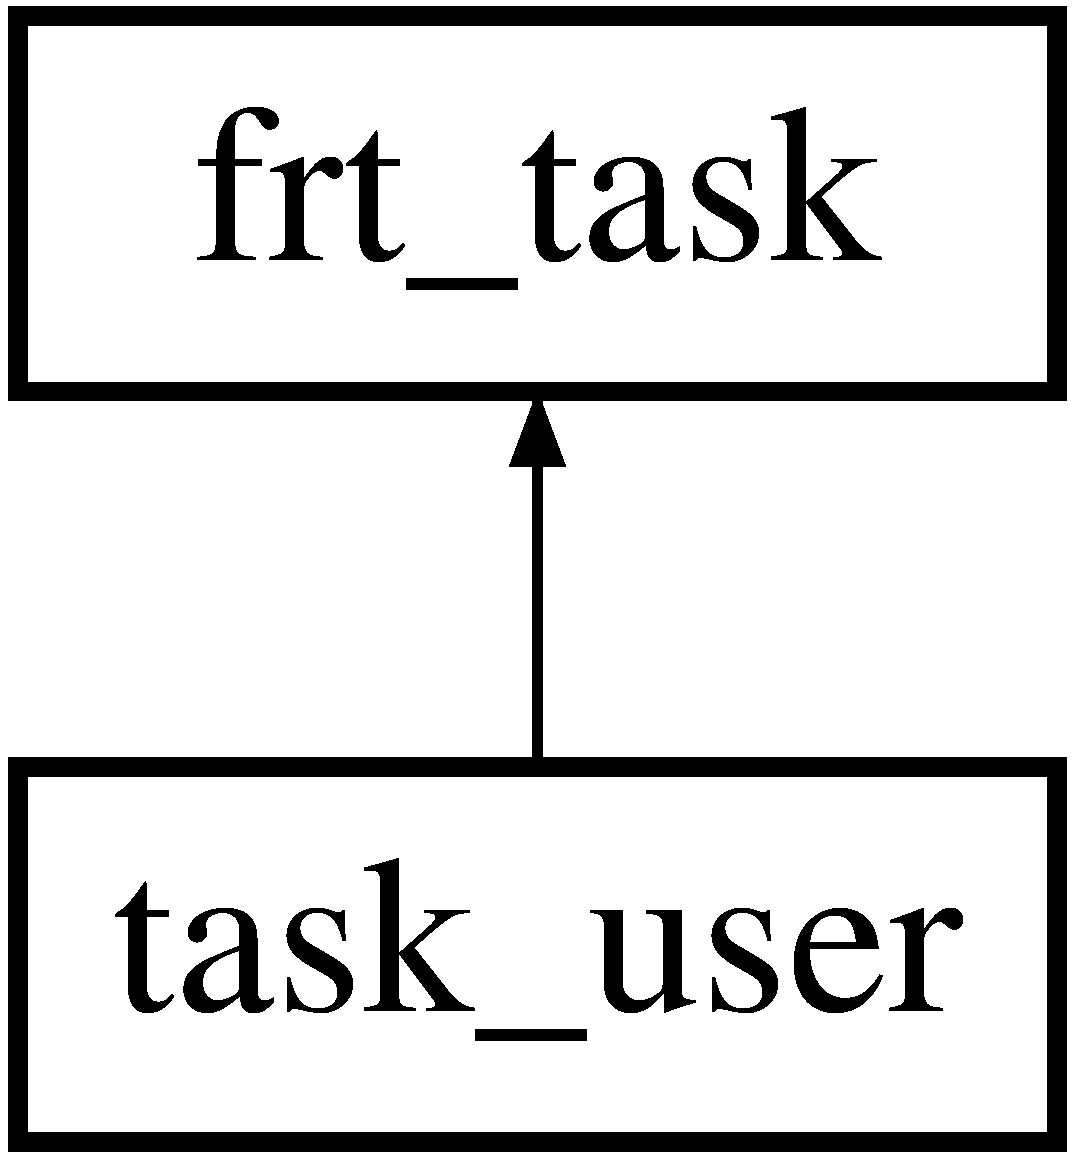
\includegraphics[height=2.000000cm]{classtask__user}
\end{center}
\end{figure}
\subsection*{Public Member Functions}
\begin{DoxyCompactItemize}
\item 
\hyperlink{classtask__user_a3aba77563b375bb14838800608da48bc}{task\+\_\+user} (const char $\ast$, unsigned port\+B\+A\+S\+E\+\_\+\+T\+Y\+P\+E, size\+\_\+t, emstream $\ast$)
\item 
void \hyperlink{classtask__user_adca6429d57be25e8d411414fc8ad75af}{run} (void)
\item 
void \hyperlink{classtask__user_a78170e5ebe8dca1ce0a5a09c507399f1}{print\+\_\+status} (emstream \&)
\end{DoxyCompactItemize}
\subsection*{Protected Member Functions}
\begin{DoxyCompactItemize}
\item 
void \hyperlink{classtask__user_a75475060f83bae1e44bcc8a5c34015c7}{print\+\_\+help\+\_\+message} (void)
\item 
void \hyperlink{classtask__user_a105bebbd9cb1031154c3dfc3662db4a0}{show\+\_\+status} (void)
\item 
void \hyperlink{classtask__user_a62e9a23d2a052ef1c34ef4c6f1152032}{motor\+\_\+menu} (void)
\item 
void \hyperlink{classtask__user_aab1a6f3f0ea7acce28c845a0cf992e6d}{motor\+\_\+settings} (void)
\end{DoxyCompactItemize}
\subsection*{Protected Attributes}
\begin{DoxyCompactItemize}
\item 
emstream $\ast$ \hyperlink{classtask__user_a04ed5c2b4d7c9a1530bde6f217e01681}{p\+\_\+serial}
\item 
\hypertarget{classtask__user_ac85973422902084fc9a4692250be32fe}{uint32\+\_\+t \hyperlink{classtask__user_ac85973422902084fc9a4692250be32fe}{runs}}\label{classtask__user_ac85973422902084fc9a4692250be32fe}

\begin{DoxyCompactList}\small\item\em This variable counts the number of runs through this task's loop. \end{DoxyCompactList}\end{DoxyCompactItemize}


\subsection{Detailed Description}
This task reads measurements that were taken by the data acquisition task in task\+\_\+daq.$\ast$ and puts those measurements into a queue. 

Definition at line 57 of file task\+\_\+user.\+h.



\subsection{Constructor \& Destructor Documentation}
\hypertarget{classtask__user_a3aba77563b375bb14838800608da48bc}{\index{task\+\_\+user@{task\+\_\+user}!task\+\_\+user@{task\+\_\+user}}
\index{task\+\_\+user@{task\+\_\+user}!task\+\_\+user@{task\+\_\+user}}
\subsubsection[{task\+\_\+user}]{\setlength{\rightskip}{0pt plus 5cm}task\+\_\+user\+::task\+\_\+user (
\begin{DoxyParamCaption}
\item[{const char $\ast$}]{a\+\_\+name, }
\item[{unsigned port\+B\+A\+S\+E\+\_\+\+T\+Y\+P\+E}]{a\+\_\+priority, }
\item[{size\+\_\+t}]{a\+\_\+stack\+\_\+size, }
\item[{emstream $\ast$}]{p\+\_\+ser\+\_\+dev}
\end{DoxyParamCaption}
)}}\label{classtask__user_a3aba77563b375bb14838800608da48bc}
This constructor creates a new data acquisition task. Its main job is to call the parent class's constructor which does most of the work. 
\begin{DoxyParams}{Parameters}
{\em a\+\_\+name} & A character string which will be the name of this task \\
\hline
{\em a\+\_\+priority} & The priority at which this task will initially run (default\+: 0) \\
\hline
{\em a\+\_\+stack\+\_\+size} & The size of this task's stack in bytes (default\+: config\+M\+I\+N\+I\+M\+A\+L\+\_\+\+S\+T\+A\+C\+K\+\_\+\+S\+I\+Z\+E) \\
\hline
{\em p\+\_\+ser\+\_\+dev} & Pointer to a serial device (port, radio, S\+D card, etc.) which can be used by this task to communicate (default\+: N\+U\+L\+L) \\
\hline
\end{DoxyParams}


Definition at line 55 of file task\+\_\+user.\+cpp.



References p\+\_\+serial, and runs.



\subsection{Member Function Documentation}
\hypertarget{classtask__user_a62e9a23d2a052ef1c34ef4c6f1152032}{\index{task\+\_\+user@{task\+\_\+user}!motor\+\_\+menu@{motor\+\_\+menu}}
\index{motor\+\_\+menu@{motor\+\_\+menu}!task\+\_\+user@{task\+\_\+user}}
\subsubsection[{motor\+\_\+menu}]{\setlength{\rightskip}{0pt plus 5cm}void task\+\_\+user\+::motor\+\_\+menu (
\begin{DoxyParamCaption}
\item[{void}]{}
\end{DoxyParamCaption}
)\hspace{0.3cm}{\ttfamily [protected]}}}\label{classtask__user_a62e9a23d2a052ef1c34ef4c6f1152032}
This method prints out the diferent options for the motor menu imlpmented in \hyperlink{classtask__user_adca6429d57be25e8d411414fc8ad75af}{run()}. It shows the possible inputs it accepts as well as what they do. 

Definition at line 241 of file task\+\_\+user.\+cpp.



References motor\+\_\+select, p\+\_\+serial, pot\+\_\+1, and pot\+\_\+2.



Referenced by motor\+\_\+settings(), and run().

\hypertarget{classtask__user_aab1a6f3f0ea7acce28c845a0cf992e6d}{\index{task\+\_\+user@{task\+\_\+user}!motor\+\_\+settings@{motor\+\_\+settings}}
\index{motor\+\_\+settings@{motor\+\_\+settings}!task\+\_\+user@{task\+\_\+user}}
\subsubsection[{motor\+\_\+settings}]{\setlength{\rightskip}{0pt plus 5cm}void task\+\_\+user\+::motor\+\_\+settings (
\begin{DoxyParamCaption}
\item[{void}]{}
\end{DoxyParamCaption}
)\hspace{0.3cm}{\ttfamily [protected]}}}\label{classtask__user_aab1a6f3f0ea7acce28c845a0cf992e6d}
This function is the implementation of the motor menu. Given correct inputs it will let you change motor, change pot state, change power settings, run the brakes, and switch back to the main menu. Incorrect input are more or less ignored 

Definition at line 261 of file task\+\_\+user.\+cpp.



References brake\+\_\+1, brake\+\_\+2, motor\+\_\+menu(), motor\+\_\+select, p\+\_\+serial, pot\+\_\+1, pot\+\_\+2, power\+\_\+1, and power\+\_\+2.



Referenced by run().

\hypertarget{classtask__user_a75475060f83bae1e44bcc8a5c34015c7}{\index{task\+\_\+user@{task\+\_\+user}!print\+\_\+help\+\_\+message@{print\+\_\+help\+\_\+message}}
\index{print\+\_\+help\+\_\+message@{print\+\_\+help\+\_\+message}!task\+\_\+user@{task\+\_\+user}}
\subsubsection[{print\+\_\+help\+\_\+message}]{\setlength{\rightskip}{0pt plus 5cm}void task\+\_\+user\+::print\+\_\+help\+\_\+message (
\begin{DoxyParamCaption}
\item[{void}]{}
\end{DoxyParamCaption}
)\hspace{0.3cm}{\ttfamily [protected]}}}\label{classtask__user_a75475060f83bae1e44bcc8a5c34015c7}
This method prints out the diferent options for the main menu imlpmented in \hyperlink{classtask__user_adca6429d57be25e8d411414fc8ad75af}{run()}. It shows the possible inputs it accepts as well as what they do. 

Definition at line 165 of file task\+\_\+user.\+cpp.



References p\+\_\+serial.



Referenced by run().

\hypertarget{classtask__user_a78170e5ebe8dca1ce0a5a09c507399f1}{\index{task\+\_\+user@{task\+\_\+user}!print\+\_\+status@{print\+\_\+status}}
\index{print\+\_\+status@{print\+\_\+status}!task\+\_\+user@{task\+\_\+user}}
\subsubsection[{print\+\_\+status}]{\setlength{\rightskip}{0pt plus 5cm}void task\+\_\+user\+::print\+\_\+status (
\begin{DoxyParamCaption}
\item[{emstream \&}]{ser\+\_\+thing}
\end{DoxyParamCaption}
)}}\label{classtask__user_a78170e5ebe8dca1ce0a5a09c507399f1}
This method prints information about the status of this task. It is called by the overloaded \char`\"{}$<$$<$\char`\"{} operator so that when the task prints itself to a serial device, whatever this method wants printed gets printed. 
\begin{DoxyParams}{Parameters}
{\em ser\+\_\+thing} & The serial device to which information will be printed \\
\hline
\end{DoxyParams}


Definition at line 228 of file task\+\_\+user.\+cpp.



References runs.

\hypertarget{classtask__user_adca6429d57be25e8d411414fc8ad75af}{\index{task\+\_\+user@{task\+\_\+user}!run@{run}}
\index{run@{run}!task\+\_\+user@{task\+\_\+user}}
\subsubsection[{run}]{\setlength{\rightskip}{0pt plus 5cm}void task\+\_\+user\+::run (
\begin{DoxyParamCaption}
\item[{void}]{}
\end{DoxyParamCaption}
)}}\label{classtask__user_adca6429d57be25e8d411414fc8ad75af}
This run method is called by the R\+T\+O\+S and contains a loop in which the task checks for user input and characters in the print queue, dealing with each in the appropriate manner.

This task is the main loop that runs the menu. You can chose options from the main menu, including printing the time, version, and stack, or you can go to the motor menu implemented in \hyperlink{classtask__user_a62e9a23d2a052ef1c34ef4c6f1152032}{motor\+\_\+menu()} 

Definition at line 76 of file task\+\_\+user.\+cpp.



References motor\+\_\+menu(), motor\+\_\+settings(), p\+\_\+serial, print\+\_\+help\+\_\+message(), print\+\_\+ser\+\_\+queue, runs, and show\+\_\+status().

\hypertarget{classtask__user_a105bebbd9cb1031154c3dfc3662db4a0}{\index{task\+\_\+user@{task\+\_\+user}!show\+\_\+status@{show\+\_\+status}}
\index{show\+\_\+status@{show\+\_\+status}!task\+\_\+user@{task\+\_\+user}}
\subsubsection[{show\+\_\+status}]{\setlength{\rightskip}{0pt plus 5cm}void task\+\_\+user\+::show\+\_\+status (
\begin{DoxyParamCaption}
\item[{void}]{}
\end{DoxyParamCaption}
)\hspace{0.3cm}{\ttfamily [protected]}}}\label{classtask__user_a105bebbd9cb1031154c3dfc3662db4a0}
This method displays information about the status of the system, including \begin{DoxyItemize}
\item The name and version of the program \item The name, status, priority, and free stack space of each task \item Processor cycles used by each task \item Amount of heap space free and setting of R\+T\+O\+S tick timer \end{DoxyItemize}


Definition at line 185 of file task\+\_\+user.\+cpp.



References p\+\_\+serial, and P\+R\+O\+G\+R\+A\+M\+\_\+\+V\+E\+R\+S\+I\+O\+N.



Referenced by run().



\subsection{Member Data Documentation}
\hypertarget{classtask__user_a04ed5c2b4d7c9a1530bde6f217e01681}{\index{task\+\_\+user@{task\+\_\+user}!p\+\_\+serial@{p\+\_\+serial}}
\index{p\+\_\+serial@{p\+\_\+serial}!task\+\_\+user@{task\+\_\+user}}
\subsubsection[{p\+\_\+serial}]{\setlength{\rightskip}{0pt plus 5cm}emstream$\ast$ task\+\_\+user\+::p\+\_\+serial\hspace{0.3cm}{\ttfamily [protected]}}}\label{classtask__user_a04ed5c2b4d7c9a1530bde6f217e01681}
This pointer allows all the methods in this task to use the serial port, or whatever serial device is being used to communicate with the user. 

Definition at line 65 of file task\+\_\+user.\+h.



Referenced by motor\+\_\+menu(), motor\+\_\+settings(), print\+\_\+help\+\_\+message(), run(), show\+\_\+status(), and task\+\_\+user().



The documentation for this class was generated from the following files\+:\begin{DoxyCompactItemize}
\item 
\hyperlink{task__user_8h}{task\+\_\+user.\+h}\item 
\hyperlink{task__user_8cpp}{task\+\_\+user.\+cpp}\end{DoxyCompactItemize}

\chapter{\-File \-Documentation}
\hypertarget{adc_8cpp}{\section{adc.\-cpp \-File \-Reference}
\label{adc_8cpp}\index{adc.\-cpp@{adc.\-cpp}}
}
{\ttfamily \#include $<$stdlib.\-h$>$}\*
{\ttfamily \#include $<$avr/io.\-h$>$}\*
{\ttfamily \#include \char`\"{}rs232int.\-h\char`\"{}}\*
{\ttfamily \#include \char`\"{}adc.\-h\char`\"{}}\*
\subsection*{\-Functions}
\begin{DoxyCompactItemize}
\item 
emstream \& \hyperlink{adc_8cpp_afb33ca9fe94765ee57079e7feb03f975}{operator$<$$<$} (emstream \&serpt, \hyperlink{classadc}{adc} \&a2d)
\begin{DoxyCompactList}\small\item\em \-This overloaded operator \char`\"{}prints\char`\"{} the \-A/\-D converter. \end{DoxyCompactList}\end{DoxyCompactItemize}


\subsection{\-Detailed \-Description}
\-This file contains a very simple \-A/\-D converter driver. \-The driver is hopefully thread safe in \-Free\-R\-T\-O\-S due to the use of a mutex to prevent its use by multiple tasks at the same time. \-There is no protection from priority inversion, however, except for the priority elevation in the mutex.

\-Revisions\-: \begin{DoxyItemize}
\item 01-\/15-\/2008 \-J\-R\-R \-Original (somewhat useful) file \item 10-\/11-\/2012 \-J\-R\-R \-Less original, more useful file with \-Free\-R\-T\-O\-S mutex added \item 10-\/12-\/2012 \-J\-R\-R \-There was a bug in the mutex code, and it has been fixed\end{DoxyItemize}
\-License\-: \-This file is copyright 2012 by \-J\-R \-Ridgely and released under the \-Lesser \-G\-N\-U \-Public \-License, version 2. \-It intended for educational use only, but its use is not limited thereto. 

\-Definition in file \hyperlink{adc_8cpp_source}{adc.\-cpp}.



\subsection{\-Function \-Documentation}
\hypertarget{adc_8cpp_afb33ca9fe94765ee57079e7feb03f975}{\index{adc.\-cpp@{adc.\-cpp}!operator$<$$<$@{operator$<$$<$}}
\index{operator$<$$<$@{operator$<$$<$}!adc.cpp@{adc.\-cpp}}
\subsubsection[{operator$<$$<$}]{\setlength{\rightskip}{0pt plus 5cm}emstream\& operator$<$$<$ (
\begin{DoxyParamCaption}
\item[{emstream \&}]{serpt, }
\item[{{\bf adc} \&}]{a2d}
\end{DoxyParamCaption}
)}}\label{adc_8cpp_afb33ca9fe94765ee57079e7feb03f975}


\-This overloaded operator \char`\"{}prints\char`\"{} the \-A/\-D converter. 

{\bfseries \-Details\-:} \-This overloaded operator will return \-A\-D\-M\-U\-X and \-A\-D\-C\-S\-R\-A in binary. 
\begin{DoxyParams}{\-Parameters}
{\em serpt} & \-The serial port where the printout will be printed. \\
\hline
{\em a2d} & \-The \-A/\-D driver which is being printed. \\
\hline
\end{DoxyParams}
\begin{DoxyReturn}{\-Returns}
\-A reference to the same serial device that the information is written to. \-This is used to string together things to write with \char`\"{}$<$$<$\char`\"{} operators 
\end{DoxyReturn}


\-Definition at line 120 of file adc.\-cpp.


\hypertarget{adc_8h}{\section{adc.\-h \-File \-Reference}
\label{adc_8h}\index{adc.\-h@{adc.\-h}}
}
{\ttfamily \#include \char`\"{}emstream.\-h\char`\"{}}\*
{\ttfamily \#include \char`\"{}\-Free\-R\-T\-O\-S.\-h\char`\"{}}\*
{\ttfamily \#include \char`\"{}task.\-h\char`\"{}}\*
{\ttfamily \#include \char`\"{}queue.\-h\char`\"{}}\*
{\ttfamily \#include \char`\"{}semphr.\-h\char`\"{}}\*
\subsection*{\-Classes}
\begin{DoxyCompactItemize}
\item 
class \hyperlink{classadc}{adc}
\begin{DoxyCompactList}\small\item\em \-This class should run the \-A/\-D converter on an \-A\-V\-R processor. \end{DoxyCompactList}\end{DoxyCompactItemize}
\subsection*{\-Functions}
\begin{DoxyCompactItemize}
\item 
emstream \& \hyperlink{adc_8h_a6e6d1e227b216fe2a1fee9b0ea52180d}{operator$<$$<$} (emstream \&, \hyperlink{classadc}{adc} \&)
\begin{DoxyCompactList}\small\item\em \-This overloaded operator \char`\"{}prints\char`\"{} the \-A/\-D converter. \end{DoxyCompactList}\end{DoxyCompactItemize}


\subsection{\-Detailed \-Description}
\-This file contains a very simple \-A/\-D converter driver. \-The driver is hopefully thread safe in \-Free\-R\-T\-O\-S due to the use of a mutex to prevent its use by multiple tasks at the same time. \-There is no protection from priority inversion, however, except for the priority elevation in the mutex.

\-Revisions\-: \begin{DoxyItemize}
\item 01-\/15-\/2008 \-J\-R\-R \-Original (somewhat useful) file \item 10-\/11-\/2012 \-J\-R\-R \-Less original, more useful file with \-Free\-R\-T\-O\-S mutex added \item 10-\/12-\/2012 \-J\-R\-R \-There was a bug in the mutex code, and it has been fixed\end{DoxyItemize}
\-License\-: \-This file is copyright 2012 by \-J\-R \-Ridgely and released under the \-Lesser \-G\-N\-U \-Public \-License, version 2. \-It intended for educational use only, but its use is not limited thereto. 

\-Definition in file \hyperlink{adc_8h_source}{adc.\-h}.



\subsection{\-Function \-Documentation}
\hypertarget{adc_8h_a6e6d1e227b216fe2a1fee9b0ea52180d}{\index{adc.\-h@{adc.\-h}!operator$<$$<$@{operator$<$$<$}}
\index{operator$<$$<$@{operator$<$$<$}!adc.h@{adc.\-h}}
\subsubsection[{operator$<$$<$}]{\setlength{\rightskip}{0pt plus 5cm}emstream\& operator$<$$<$ (
\begin{DoxyParamCaption}
\item[{emstream \&}]{serpt, }
\item[{{\bf adc} \&}]{a2d}
\end{DoxyParamCaption}
)}}\label{adc_8h_a6e6d1e227b216fe2a1fee9b0ea52180d}


\-This overloaded operator \char`\"{}prints\char`\"{} the \-A/\-D converter. 

{\bfseries \-Details\-:} \-This overloaded operator will return \-A\-D\-M\-U\-X and \-A\-D\-C\-S\-R\-A in binary. 
\begin{DoxyParams}{\-Parameters}
{\em serpt} & \-The serial port where the printout will be printed. \\
\hline
{\em a2d} & \-The \-A/\-D driver which is being printed. \\
\hline
\end{DoxyParams}
\begin{DoxyReturn}{\-Returns}
\-A reference to the same serial device that the information is written to. \-This is used to string together things to write with \char`\"{}$<$$<$\char`\"{} operators 
\end{DoxyReturn}


\-Definition at line 120 of file adc.\-cpp.


\hypertarget{motor__driver_8cpp}{\section{motor\-\_\-driver.\-cpp \-File \-Reference}
\label{motor__driver_8cpp}\index{motor\-\_\-driver.\-cpp@{motor\-\_\-driver.\-cpp}}
}
{\ttfamily \#include $<$stdlib.\-h$>$}\*
{\ttfamily \#include $<$avr/io.\-h$>$}\*
{\ttfamily \#include \char`\"{}rs232int.\-h\char`\"{}}\*
{\ttfamily \#include \char`\"{}motor\-\_\-driver.\-h\char`\"{}}\*


\subsection{\-Detailed \-Description}
\-This file contains a very simple motor driver. \-This driver should be used to provide power to a moter, varrying in strenth by changing the pwm, as well as a full out breaking function. 

\-Definition in file \hyperlink{motor__driver_8cpp_source}{motor\-\_\-driver.\-cpp}.


\hypertarget{motor__driver_8h}{\section{motor\-\_\-driver.\-h \-File \-Reference}
\label{motor__driver_8h}\index{motor\-\_\-driver.\-h@{motor\-\_\-driver.\-h}}
}
{\ttfamily \#include \char`\"{}emstream.\-h\char`\"{}}\*
{\ttfamily \#include \char`\"{}\-Free\-R\-T\-O\-S.\-h\char`\"{}}\*
{\ttfamily \#include \char`\"{}task.\-h\char`\"{}}\*
{\ttfamily \#include \char`\"{}queue.\-h\char`\"{}}\*
{\ttfamily \#include \char`\"{}semphr.\-h\char`\"{}}\*
\subsection*{\-Classes}
\begin{DoxyCompactItemize}
\item 
class \hyperlink{classmotor__driver}{motor\-\_\-driver}
\begin{DoxyCompactList}\small\item\em \-This class runs the motor on the h-\/bridge chip. \end{DoxyCompactList}\end{DoxyCompactItemize}


\subsection{\-Detailed \-Description}
\-This file provides the creation and interface for running a simple motor. \-You can change the power, which will take you from full forward to full reverse. \-If you put the power at half it will freewheel. \-You can also break at any time. 

\-Definition in file \hyperlink{motor__driver_8h_source}{motor\-\_\-driver.\-h}.


\hypertarget{shares_8h}{\section{shares.\+h File Reference}
\label{shares_8h}\index{shares.\+h@{shares.\+h}}
}
\subsection*{Variables}
\begin{DoxyCompactItemize}
\item 
frt\+\_\+text\+\_\+queue $\ast$ \hyperlink{shares_8h_a0f3e0982ec5df30e2339e7162f60a1d6}{print\+\_\+ser\+\_\+queue}
\item 
frt\+\_\+queue$<$ uint32\+\_\+t $>$ $\ast$ \hyperlink{shares_8h_a943b100cc398890af64c8c00626935cd}{p\+\_\+queue\+\_\+1}
\item 
shared\+\_\+data$<$ uint32\+\_\+t $>$ $\ast$ \hyperlink{shares_8h_a6e36343e3fbd1317e9bbbdfee0691141}{p\+\_\+share\+\_\+1}
\item 
uint32\+\_\+t $\ast$ \hyperlink{shares_8h_a72ac6f1f6a1b9cb1edc7836f31af85b5}{p\+\_\+glob\+\_\+of\+\_\+probs}
\item 
shared\+\_\+data$<$ float $>$ $\ast$ \hyperlink{shares_8h_ac174d5bcd10a2ba8775bab06712b7ce8}{p\+\_\+rate\+\_\+1}
\end{DoxyCompactItemize}


\subsection{Detailed Description}
This file contains extern declarations for queues and other inter-\/task data communication objects used in a M\+E405/507/\+Free\+R\+T\+O\+S project.

Revisions\+: \begin{DoxyItemize}
\item 09-\/30-\/2012 J\+R\+R Original file was a one-\/file demonstration with two tasks \item 10-\/05-\/2012 J\+R\+R Split into multiple files, one for each task plus a main one \item 10-\/29-\/2012 J\+R\+R Reorganized with global queue and shared data references\end{DoxyItemize}
License\+: This file is copyright 2012 by J\+R Ridgely and released under the Lesser G\+N\+U Public License, version 2. It intended for educational use only, but its use is not limited thereto. 

Definition in file \hyperlink{shares_8h_source}{shares.\+h}.



\subsection{Variable Documentation}
\hypertarget{shares_8h_a72ac6f1f6a1b9cb1edc7836f31af85b5}{\index{shares.\+h@{shares.\+h}!p\+\_\+glob\+\_\+of\+\_\+probs@{p\+\_\+glob\+\_\+of\+\_\+probs}}
\index{p\+\_\+glob\+\_\+of\+\_\+probs@{p\+\_\+glob\+\_\+of\+\_\+probs}!shares.\+h@{shares.\+h}}
\subsubsection[{p\+\_\+glob\+\_\+of\+\_\+probs}]{\setlength{\rightskip}{0pt plus 5cm}uint32\+\_\+t$\ast$ p\+\_\+glob\+\_\+of\+\_\+probs}}\label{shares_8h_a72ac6f1f6a1b9cb1edc7836f31af85b5}
This global variable will be written by the source task and read by the sink task. We expect the process to be corrupted by context switches now and then. 

Definition at line 89 of file test\+\_\+main.\+cpp.



Referenced by main(), task\+\_\+sink\+::run(), and task\+\_\+source\+::run().

\hypertarget{shares_8h_a943b100cc398890af64c8c00626935cd}{\index{shares.\+h@{shares.\+h}!p\+\_\+queue\+\_\+1@{p\+\_\+queue\+\_\+1}}
\index{p\+\_\+queue\+\_\+1@{p\+\_\+queue\+\_\+1}!shares.\+h@{shares.\+h}}
\subsubsection[{p\+\_\+queue\+\_\+1}]{\setlength{\rightskip}{0pt plus 5cm}frt\+\_\+queue$<$uint32\+\_\+t$>$$\ast$ p\+\_\+queue\+\_\+1}}\label{shares_8h_a943b100cc398890af64c8c00626935cd}
This queue sends data from the source task to the sink task. 

Definition at line 79 of file test\+\_\+main.\+cpp.



Referenced by main(), task\+\_\+sink\+::run(), and task\+\_\+source\+::run().

\hypertarget{shares_8h_ac174d5bcd10a2ba8775bab06712b7ce8}{\index{shares.\+h@{shares.\+h}!p\+\_\+rate\+\_\+1@{p\+\_\+rate\+\_\+1}}
\index{p\+\_\+rate\+\_\+1@{p\+\_\+rate\+\_\+1}!shares.\+h@{shares.\+h}}
\subsubsection[{p\+\_\+rate\+\_\+1}]{\setlength{\rightskip}{0pt plus 5cm}shared\+\_\+data$<$float$>$$\ast$ p\+\_\+rate\+\_\+1}}\label{shares_8h_ac174d5bcd10a2ba8775bab06712b7ce8}
This shared data item is used by the time rate measurement task to make its measurements of how fast something is happening available to other tasks. 

Definition at line 94 of file test\+\_\+main.\+cpp.



Referenced by main().

\hypertarget{shares_8h_a6e36343e3fbd1317e9bbbdfee0691141}{\index{shares.\+h@{shares.\+h}!p\+\_\+share\+\_\+1@{p\+\_\+share\+\_\+1}}
\index{p\+\_\+share\+\_\+1@{p\+\_\+share\+\_\+1}!shares.\+h@{shares.\+h}}
\subsubsection[{p\+\_\+share\+\_\+1}]{\setlength{\rightskip}{0pt plus 5cm}shared\+\_\+data$<$uint32\+\_\+t$>$$\ast$ p\+\_\+share\+\_\+1}}\label{shares_8h_a6e36343e3fbd1317e9bbbdfee0691141}
This shared data item allows a value to be posted by the source task and read by the sink task. 

Definition at line 84 of file test\+\_\+main.\+cpp.



Referenced by main(), task\+\_\+sink\+::run(), and task\+\_\+source\+::run().

\hypertarget{shares_8h_a0f3e0982ec5df30e2339e7162f60a1d6}{\index{shares.\+h@{shares.\+h}!print\+\_\+ser\+\_\+queue@{print\+\_\+ser\+\_\+queue}}
\index{print\+\_\+ser\+\_\+queue@{print\+\_\+ser\+\_\+queue}!shares.\+h@{shares.\+h}}
\subsubsection[{print\+\_\+ser\+\_\+queue}]{\setlength{\rightskip}{0pt plus 5cm}frt\+\_\+text\+\_\+queue$\ast$ print\+\_\+ser\+\_\+queue}}\label{shares_8h_a0f3e0982ec5df30e2339e7162f60a1d6}
This is a print queue, descended from base\+\_\+text\+\_\+serial so that things can be printed into the queue using the \char`\"{}$<$$<$\char`\"{} operator and they'll come out the other end as a stream of characters. It's used by tasks that send things to the user interface task to be printed. 

Definition at line 75 of file test\+\_\+main.\+cpp.



Referenced by main(), task\+\_\+sink\+::run(), task\+\_\+user\+::run(), and task\+\_\+sink\+::show\+\_\+errors().


\hypertarget{task__multi_8cpp}{\section{task\+\_\+multi.\+cpp File Reference}
\label{task__multi_8cpp}\index{task\+\_\+multi.\+cpp@{task\+\_\+multi.\+cpp}}
}
{\ttfamily \#include \char`\"{}frt\+\_\+text\+\_\+queue.\+h\char`\"{}}\\*
{\ttfamily \#include \char`\"{}task\+\_\+multi.\+h\char`\"{}}\\*
{\ttfamily \#include \char`\"{}shares.\+h\char`\"{}}\\*


\subsection{Detailed Description}
This file contains the code for a task class which will be instantiated many times to test how many tasks can be safely run on various A\+V\+R processors using the M\+E507/\+Free\+R\+T\+O\+S software.

Revisions\+: \begin{DoxyItemize}
\item 09-\/30-\/2012 J\+R\+R Original file was a one-\/file demonstration with two tasks \item 10-\/05-\/2012 J\+R\+R Split into multiple files, one for each task \item 10-\/25-\/2012 J\+R\+R Changed to a more fully C++ version with class task\+\_\+sender \item 10-\/27-\/2012 J\+R\+R Altered from data sending task into L\+E\+D blinking class \item 11-\/04-\/2012 J\+R\+R Altered again into the multi-\/task monstrosity\end{DoxyItemize}
License\+: This file is copyright 2012 by J\+R Ridgely and released under the Lesser G\+N\+U Public License, version 2. It intended for educational use only, but its use is not limited thereto. 

Definition in file \hyperlink{task__multi_8cpp_source}{task\+\_\+multi.\+cpp}.


\hypertarget{task__multi_8h}{\section{task\-\_\-multi.\-h \-File \-Reference}
\label{task__multi_8h}\index{task\-\_\-multi.\-h@{task\-\_\-multi.\-h}}
}
{\ttfamily \#include $<$stdlib.\-h$>$}\*
{\ttfamily \#include \char`\"{}\-Free\-R\-T\-O\-S.\-h\char`\"{}}\*
{\ttfamily \#include \char`\"{}task.\-h\char`\"{}}\*
{\ttfamily \#include \char`\"{}queue.\-h\char`\"{}}\*
{\ttfamily \#include \char`\"{}frt\-\_\-task.\-h\char`\"{}}\*
{\ttfamily \#include \char`\"{}rs232int.\-h\char`\"{}}\*
{\ttfamily \#include \char`\"{}time\-\_\-stamp.\-h\char`\"{}}\*
{\ttfamily \#include \char`\"{}frt\-\_\-queue.\-h\char`\"{}}\*
{\ttfamily \#include \char`\"{}frt\-\_\-shared\-\_\-data.\-h\char`\"{}}\*
\subsection*{\-Classes}
\begin{DoxyCompactItemize}
\item 
class \hyperlink{classtask__multi}{task\-\_\-multi}
\end{DoxyCompactItemize}


\subsection{\-Detailed \-Description}
\-This file contains the header for a task class which is will be instantiated many times to test how many tasks can be safely run on various \-A\-V\-R processors using the \-M\-E507/\-Free\-R\-T\-O\-S software.

\-Revisions\-: \begin{DoxyItemize}
\item 09-\/30-\/2012 \-J\-R\-R \-Original file was a one-\/file demonstration with two tasks \item 10-\/05-\/2012 \-J\-R\-R \-Split into multiple files, one for each task \item 10-\/25-\/2012 \-J\-R\-R \-Changed to a more fully \-C++ version with class task\-\_\-sender \item 10-\/27-\/2012 \-J\-R\-R \-Altered from data sending task into \-L\-E\-D blinking class \item 11-\/04-\/2012 \-J\-R\-R \-Altered again into the multi-\/task monstrosity\end{DoxyItemize}
\-License\-: \-This file is copyright 2012 by \-J\-R \-Ridgely and released under the \-Lesser \-G\-N\-U \-Public \-License, version 2. \-It intended for educational use only, but its use is not limited thereto. 

\-Definition in file \hyperlink{task__multi_8h_source}{task\-\_\-multi.\-h}.


\hypertarget{task__sink_8cpp}{\section{task\-\_\-sink.\-cpp \-File \-Reference}
\label{task__sink_8cpp}\index{task\-\_\-sink.\-cpp@{task\-\_\-sink.\-cpp}}
}
{\ttfamily \#include \char`\"{}task\-\_\-source.\-h\char`\"{}}\*
{\ttfamily \#include \char`\"{}task\-\_\-sink.\-h\char`\"{}}\*


\subsection{\-Detailed \-Description}
\-This file contains the source code for a task which receives data via a queue, a shared data item, and a dangerous global variable so that the data may be checked for errors in transmission.

\-Revisions\-: \begin{DoxyItemize}
\item 09-\/30-\/2012 \-J\-R\-R \-Original file was a one-\/file demonstration with two tasks \item 10-\/05-\/2012 \-J\-R\-R \-Split into multiple files, one for each task \item 10-\/25-\/2012 \-J\-R\-R \-Changed to a more fully \-C++ version with class task\-\_\-sender \item 11-\/03-\/2012 \-J\-R\-R \-Morphed again into a data sink task with error checks\end{DoxyItemize}
\-License\-: \-This file is copyright 2012 by \-J\-R \-Ridgely and released under the \-Lesser \-G\-N\-U \-Public \-License, version 2. \-It intended for educational use only, but its use is not limited thereto. 

\-Definition in file \hyperlink{task__sink_8cpp_source}{task\-\_\-sink.\-cpp}.


\hypertarget{task__sink_8h}{\section{task\-\_\-sink.\-h \-File \-Reference}
\label{task__sink_8h}\index{task\-\_\-sink.\-h@{task\-\_\-sink.\-h}}
}
{\ttfamily \#include $<$stdlib.\-h$>$}\*
{\ttfamily \#include \char`\"{}\-Free\-R\-T\-O\-S.\-h\char`\"{}}\*
{\ttfamily \#include \char`\"{}task.\-h\char`\"{}}\*
{\ttfamily \#include \char`\"{}queue.\-h\char`\"{}}\*
{\ttfamily \#include \char`\"{}rs232int.\-h\char`\"{}}\*
{\ttfamily \#include \char`\"{}time\-\_\-stamp.\-h\char`\"{}}\*
{\ttfamily \#include \char`\"{}frt\-\_\-queue.\-h\char`\"{}}\*
{\ttfamily \#include \char`\"{}frt\-\_\-text\-\_\-queue.\-h\char`\"{}}\*
{\ttfamily \#include \char`\"{}frt\-\_\-shared\-\_\-data.\-h\char`\"{}}\*
{\ttfamily \#include \char`\"{}shares.\-h\char`\"{}}\*
\subsection*{\-Classes}
\begin{DoxyCompactItemize}
\item 
class \hyperlink{classtask__sink}{task\-\_\-sink}
\end{DoxyCompactItemize}


\subsection{\-Detailed \-Description}
\-This file contains the source code for a task which receives data via a queue, a shared data item, and a dangerous global variable so that the data may be checked for errors in transmission.

\-Revisions\-: \begin{DoxyItemize}
\item 09-\/30-\/2012 \-J\-R\-R \-Original file was a one-\/file demonstration with two tasks \item 10-\/05-\/2012 \-J\-R\-R \-Split into multiple files, one for each task \item 10-\/25-\/2012 \-J\-R\-R \-Changed to a more fully \-C++ version with class task\-\_\-sender \item 11-\/03-\/2012 \-J\-R\-R \-Morphed again into a data sink task with error checks\end{DoxyItemize}
\-License\-: \-This file is copyright 2012 by \-J\-R \-Ridgely and released under the \-Lesser \-G\-N\-U \-Public \-License, version 2. \-It intended for educational use only, but its use is not limited thereto. 

\-Definition in file \hyperlink{task__sink_8h_source}{task\-\_\-sink.\-h}.


\hypertarget{task__source_8cpp}{\section{task\-\_\-source.\-cpp \-File \-Reference}
\label{task__source_8cpp}\index{task\-\_\-source.\-cpp@{task\-\_\-source.\-cpp}}
}
{\ttfamily \#include \char`\"{}task\-\_\-user.\-h\char`\"{}}\*
{\ttfamily \#include \char`\"{}task\-\_\-source.\-h\char`\"{}}\*


\subsection{\-Detailed \-Description}
\-This file contains the header for a task which sends test data to another task, the data sink task, using a queue, a shared data class object, and a dangerous global variable. \-The data will be checked to test the reliability of each method of conveying the information.

\-Revisions\-: \begin{DoxyItemize}
\item 09-\/30-\/2012 \-J\-R\-R \-Original file was a one-\/file demonstration with two tasks \item 10-\/05-\/2012 \-J\-R\-R \-Split into multiple files, one for each task \item 11-\/04-\/2012 \-J\-R\-R \-Changed into the test data source task\end{DoxyItemize}
\-License\-: \-This file is copyright 2012 by \-J\-R \-Ridgely and released under the \-Lesser \-G\-N\-U \-Public \-License, version 2. \-It intended for educational use only, but its use is not limited thereto. 

\-Definition in file \hyperlink{task__source_8cpp_source}{task\-\_\-source.\-cpp}.


\hypertarget{task__source_8h}{\section{task\-\_\-source.\-h \-File \-Reference}
\label{task__source_8h}\index{task\-\_\-source.\-h@{task\-\_\-source.\-h}}
}
{\ttfamily \#include $<$stdlib.\-h$>$}\*
{\ttfamily \#include \char`\"{}\-Free\-R\-T\-O\-S.\-h\char`\"{}}\*
{\ttfamily \#include \char`\"{}task.\-h\char`\"{}}\*
{\ttfamily \#include \char`\"{}queue.\-h\char`\"{}}\*
{\ttfamily \#include \char`\"{}rs232int.\-h\char`\"{}}\*
{\ttfamily \#include \char`\"{}time\-\_\-stamp.\-h\char`\"{}}\*
{\ttfamily \#include \char`\"{}frt\-\_\-task.\-h\char`\"{}}\*
{\ttfamily \#include \char`\"{}frt\-\_\-queue.\-h\char`\"{}}\*
{\ttfamily \#include \char`\"{}frt\-\_\-text\-\_\-queue.\-h\char`\"{}}\*
{\ttfamily \#include \char`\"{}frt\-\_\-shared\-\_\-data.\-h\char`\"{}}\*
{\ttfamily \#include \char`\"{}shares.\-h\char`\"{}}\*
\subsection*{\-Classes}
\begin{DoxyCompactItemize}
\item 
class \hyperlink{classtask__source}{task\-\_\-source}
\end{DoxyCompactItemize}
\subsection*{\-Variables}
\begin{DoxyCompactItemize}
\item 
const port\-Tick\-Type \hyperlink{task__source_8h_ab24af5f6e613475c5532218fe73d0cde}{\-D\-E\-F\-\_\-\-T\-I\-C\-K\-S\-\_\-\-P\-E\-R\-\_\-\-R\-U\-N} = config\-T\-I\-C\-K\-\_\-\-R\-A\-T\-E\-\_\-\-H\-Z
\end{DoxyCompactItemize}


\subsection{\-Detailed \-Description}
\-This file contains the header for a task which sends test data to another task, the data sink task, using a queue, a shared data class object, and a dangerous global variable. \-The data will be checked to test the reliability of each method of conveying the information.

\-Revisions\-: \begin{DoxyItemize}
\item 09-\/30-\/2012 \-J\-R\-R \-Original file was a one-\/file demonstration with two tasks \item 10-\/05-\/2012 \-J\-R\-R \-Split into multiple files, one for each task \item 11-\/04-\/2012 \-J\-R\-R \-Changed into the test data source task\end{DoxyItemize}
\-License\-: \-This file is copyright 2012 by \-J\-R \-Ridgely and released under the \-Lesser \-G\-N\-U \-Public \-License, version 2. \-It intended for educational use only, but its use is not limited thereto. 

\-Definition in file \hyperlink{task__source_8h_source}{task\-\_\-source.\-h}.



\subsection{\-Variable \-Documentation}
\hypertarget{task__source_8h_ab24af5f6e613475c5532218fe73d0cde}{\index{task\-\_\-source.\-h@{task\-\_\-source.\-h}!\-D\-E\-F\-\_\-\-T\-I\-C\-K\-S\-\_\-\-P\-E\-R\-\_\-\-R\-U\-N@{\-D\-E\-F\-\_\-\-T\-I\-C\-K\-S\-\_\-\-P\-E\-R\-\_\-\-R\-U\-N}}
\index{\-D\-E\-F\-\_\-\-T\-I\-C\-K\-S\-\_\-\-P\-E\-R\-\_\-\-R\-U\-N@{\-D\-E\-F\-\_\-\-T\-I\-C\-K\-S\-\_\-\-P\-E\-R\-\_\-\-R\-U\-N}!task_source.h@{task\-\_\-source.\-h}}
\subsubsection[{\-D\-E\-F\-\_\-\-T\-I\-C\-K\-S\-\_\-\-P\-E\-R\-\_\-\-R\-U\-N}]{\setlength{\rightskip}{0pt plus 5cm}const port\-Tick\-Type {\bf \-D\-E\-F\-\_\-\-T\-I\-C\-K\-S\-\_\-\-P\-E\-R\-\_\-\-R\-U\-N} = config\-T\-I\-C\-K\-\_\-\-R\-A\-T\-E\-\_\-\-H\-Z}}\label{task__source_8h_ab24af5f6e613475c5532218fe73d0cde}
\-This is the default number of \-R\-T\-O\-S ticks per run of this task. \-If this constant is set to 100, for example, and the \-R\-T\-O\-S clock runs at 1000 \-Hz, then this task will run 10 times per second. \-This is the default value used at program startup; it's copied into a variable so that the rate of this task can be varied as needed. 

\-Definition at line 54 of file task\-\_\-source.\-h.


\hypertarget{task__user_8cpp}{\section{task\+\_\+user.\+cpp File Reference}
\label{task__user_8cpp}\index{task\+\_\+user.\+cpp@{task\+\_\+user.\+cpp}}
}
{\ttfamily \#include $<$avr/io.\+h$>$}\\*
{\ttfamily \#include $<$avr/wdt.\+h$>$}\\*
{\ttfamily \#include \char`\"{}n\+R\+F24\+L01\+\_\+text.\+h\char`\"{}}\\*
{\ttfamily \#include \char`\"{}task\+\_\+user.\+h\char`\"{}}\\*
\subsection*{Variables}
\begin{DoxyCompactItemize}
\item 
const port\+Tick\+Type \hyperlink{task__user_8cpp_a80f7a5c45b5679c45dd218506ab058f0}{ticks\+\_\+to\+\_\+delay} = ((config\+T\+I\+C\+K\+\_\+\+R\+A\+T\+E\+\_\+\+H\+Z / 1000) $\ast$ 5)
\end{DoxyCompactItemize}


\subsection{Detailed Description}
This file contains source code for a user interface task for a M\+E507/\+Free\+R\+T\+O\+S test suite.

Revisions\+: \begin{DoxyItemize}
\item 09-\/30-\/2012 J\+R\+R Original file was a one-\/file demonstration with two tasks \item 10-\/05-\/2012 J\+R\+R Split into multiple files, one for each task \item 10-\/25-\/2012 J\+R\+R Changed to a more fully C++ version with class \hyperlink{classtask__user}{task\+\_\+user} \item 11-\/04-\/2012 J\+R\+R Modified from the data acquisition example to the test suite\end{DoxyItemize}
License\+: This file is copyright 2012 by J\+R Ridgely and released under the Lesser G\+N\+U Public License, version 2. It intended for educational use only, but its use is not limited thereto. 

Definition in file \hyperlink{task__user_8cpp_source}{task\+\_\+user.\+cpp}.



\subsection{Variable Documentation}
\hypertarget{task__user_8cpp_a80f7a5c45b5679c45dd218506ab058f0}{\index{task\+\_\+user.\+cpp@{task\+\_\+user.\+cpp}!ticks\+\_\+to\+\_\+delay@{ticks\+\_\+to\+\_\+delay}}
\index{ticks\+\_\+to\+\_\+delay@{ticks\+\_\+to\+\_\+delay}!task\+\_\+user.\+cpp@{task\+\_\+user.\+cpp}}
\subsubsection[{ticks\+\_\+to\+\_\+delay}]{\setlength{\rightskip}{0pt plus 5cm}const port\+Tick\+Type ticks\+\_\+to\+\_\+delay = ((config\+T\+I\+C\+K\+\_\+\+R\+A\+T\+E\+\_\+\+H\+Z / 1000) $\ast$ 5)}}\label{task__user_8cpp_a80f7a5c45b5679c45dd218506ab058f0}
This constant sets how many R\+T\+O\+S ticks the task delays if the user's not talking. The duration is calculated to be about 5 ms. 

Definition at line 39 of file task\+\_\+user.\+cpp.


\hypertarget{task__user_8h}{\section{task\+\_\+user.\+h File Reference}
\label{task__user_8h}\index{task\+\_\+user.\+h@{task\+\_\+user.\+h}}
}
{\ttfamily \#include $<$stdlib.\+h$>$}\\*
{\ttfamily \#include \char`\"{}Free\+R\+T\+O\+S.\+h\char`\"{}}\\*
{\ttfamily \#include \char`\"{}task.\+h\char`\"{}}\\*
{\ttfamily \#include \char`\"{}queue.\+h\char`\"{}}\\*
{\ttfamily \#include \char`\"{}rs232int.\+h\char`\"{}}\\*
{\ttfamily \#include \char`\"{}time\+\_\+stamp.\+h\char`\"{}}\\*
{\ttfamily \#include \char`\"{}frt\+\_\+task.\+h\char`\"{}}\\*
{\ttfamily \#include \char`\"{}frt\+\_\+queue.\+h\char`\"{}}\\*
{\ttfamily \#include \char`\"{}frt\+\_\+text\+\_\+queue.\+h\char`\"{}}\\*
{\ttfamily \#include \char`\"{}frt\+\_\+shared\+\_\+data.\+h\char`\"{}}\\*
{\ttfamily \#include \char`\"{}shares.\+h\char`\"{}}\\*
\subsection*{Classes}
\begin{DoxyCompactItemize}
\item 
class \hyperlink{classtask__user}{task\+\_\+user}
\end{DoxyCompactItemize}
\subsection*{Macros}
\begin{DoxyCompactItemize}
\item 
\hypertarget{task__user_8h_a2f10abd650e471fae2d7e8c63d41206a}{\#define \hyperlink{task__user_8h_a2f10abd650e471fae2d7e8c63d41206a}{P\+R\+O\+G\+R\+A\+M\+\_\+\+V\+E\+R\+S\+I\+O\+N}~P\+M\+S (\char`\"{}Poly\+D\+A\+Q/Free\+R\+T\+O\+S Test V0.\+2 \char`\"{})}\label{task__user_8h_a2f10abd650e471fae2d7e8c63d41206a}

\begin{DoxyCompactList}\small\item\em This macro defines a string that identifies the name and version of this program. \end{DoxyCompactList}\end{DoxyCompactItemize}


\subsection{Detailed Description}
This file contains header stuff for a user interface task for a M\+E507/\+Free\+R\+T\+O\+S test suite.

Revisions\+: \begin{DoxyItemize}
\item 09-\/30-\/2012 J\+R\+R Original file was a one-\/file demonstration with two tasks \item 10-\/05-\/2012 J\+R\+R Split into multiple files, one for each task \item 10-\/25-\/2012 J\+R\+R Changed to a more fully C++ version with class \hyperlink{classtask__user}{task\+\_\+user} \item 11-\/04-\/2012 J\+R\+R Modified from the data acquisition example to the test suite\end{DoxyItemize}
License\+: This file is copyright 2012 by J\+R Ridgely and released under the Lesser G\+N\+U Public License, version 2. It intended for educational use only, but its use is not limited thereto. 

Definition in file \hyperlink{task__user_8h_source}{task\+\_\+user.\+h}.


\hypertarget{test__main_8cpp}{\section{test\-\_\-main.\-cpp \-File \-Reference}
\label{test__main_8cpp}\index{test\-\_\-main.\-cpp@{test\-\_\-main.\-cpp}}
}
{\ttfamily \#include $<$stdlib.\-h$>$}\*
{\ttfamily \#include $<$avr/io.\-h$>$}\*
{\ttfamily \#include $<$avr/wdt.\-h$>$}\*
{\ttfamily \#include $<$string.\-h$>$}\*
{\ttfamily \#include \char`\"{}\-Free\-R\-T\-O\-S.\-h\char`\"{}}\*
{\ttfamily \#include \char`\"{}task.\-h\char`\"{}}\*
{\ttfamily \#include \char`\"{}queue.\-h\char`\"{}}\*
{\ttfamily \#include \char`\"{}croutine.\-h\char`\"{}}\*
{\ttfamily \#include \char`\"{}rs232int.\-h\char`\"{}}\*
{\ttfamily \#include \char`\"{}time\-\_\-stamp.\-h\char`\"{}}\*
{\ttfamily \#include \char`\"{}frt\-\_\-task.\-h\char`\"{}}\*
{\ttfamily \#include \char`\"{}frt\-\_\-text\-\_\-queue.\-h\char`\"{}}\*
{\ttfamily \#include \char`\"{}frt\-\_\-queue.\-h\char`\"{}}\*
{\ttfamily \#include \char`\"{}frt\-\_\-shared\-\_\-data.\-h\char`\"{}}\*
{\ttfamily \#include \char`\"{}shares.\-h\char`\"{}}\*
{\ttfamily \#include \char`\"{}task\-\_\-user.\-h\char`\"{}}\*
{\ttfamily \#include \char`\"{}task\-\_\-motor.\-h\char`\"{}}\*
\subsection*{\-Functions}
\begin{DoxyCompactItemize}
\item 
int \hyperlink{test__main_8cpp_a840291bc02cba5474a4cb46a9b9566fe}{main} (void)
\end{DoxyCompactItemize}
\subsection*{\-Variables}
\begin{DoxyCompactItemize}
\item 
const uint8\-\_\-t \hyperlink{test__main_8cpp_a6dd5794690e811f62bce8432acff99a0}{\-N\-\_\-\-M\-U\-L\-T\-I\-\_\-\-T\-A\-S\-K\-S} = 4
\item 
frt\-\_\-text\-\_\-queue $\ast$ \hyperlink{test__main_8cpp_a0f3e0982ec5df30e2339e7162f60a1d6}{print\-\_\-ser\-\_\-queue}
\item 
frt\-\_\-queue$<$ uint32\-\_\-t $>$ $\ast$ \hyperlink{test__main_8cpp_a943b100cc398890af64c8c00626935cd}{p\-\_\-queue\-\_\-1}
\item 
shared\-\_\-data$<$ uint32\-\_\-t $>$ $\ast$ \hyperlink{test__main_8cpp_a6e36343e3fbd1317e9bbbdfee0691141}{p\-\_\-share\-\_\-1}
\item 
shared\-\_\-data$<$ int16\-\_\-t $>$ $\ast$ \hyperlink{test__main_8cpp_af4072aaf6ada6eb77990a94e7635f3cf}{power\-\_\-1}
\item 
shared\-\_\-data$<$ int16\-\_\-t $>$ $\ast$ \hyperlink{test__main_8cpp_a083156cd9b0019a19d58e68339029490}{power\-\_\-2}
\item 
shared\-\_\-data$<$ bool $>$ $\ast$ \hyperlink{test__main_8cpp_ac332aa182be3f396aab006e2a1223a8d}{brake\-\_\-1}
\item 
shared\-\_\-data$<$ bool $>$ $\ast$ \hyperlink{test__main_8cpp_a97c4fd12a21fba2f57e184c9132f2a80}{brake\-\_\-2}
\item 
shared\-\_\-data$<$ bool $>$ $\ast$ \hyperlink{test__main_8cpp_aa5a892890ce4839648694e817fbddfd3}{pot\-\_\-1}
\item 
shared\-\_\-data$<$ bool $>$ $\ast$ \hyperlink{test__main_8cpp_a67de327568f25bf830e7d71505443de8}{pot\-\_\-2}
\item 
uint32\-\_\-t $\ast$ \hyperlink{test__main_8cpp_a72ac6f1f6a1b9cb1edc7836f31af85b5}{p\-\_\-glob\-\_\-of\-\_\-probs}
\item 
shared\-\_\-data$<$ float $>$ $\ast$ \hyperlink{test__main_8cpp_ac174d5bcd10a2ba8775bab06712b7ce8}{p\-\_\-rate\-\_\-1}
\end{DoxyCompactItemize}


\subsection{\-Detailed \-Description}
\-This file contains the \hyperlink{test__main_8cpp_a840291bc02cba5474a4cb46a9b9566fe}{main()} code for a program which tests various features of the \-M\-E405/\-M\-E507/\-Free\-R\-T\-O\-S software package. \-Tests include sending data from tasks to other tasks by several means and checking for errors in transmission; creating large numbers of tasks and getting them to all run at the same time; and testing time stamps by measuring the frequency of signals sent by a signal generator.

\-Revisions\-: \begin{DoxyItemize}
\item 09-\/30-\/2012 \-J\-R\-R \-Original file was a one-\/file demonstration with two tasks \item 10-\/05-\/2012 \-J\-R\-R \-Split into multiple files, one for each task plus a main one \item 10-\/30-\/2012 \-J\-R\-R \-A hopefully somewhat stable version with global queue pointers and the new operator used for most memory allocation \item 11-\/04-\/2012 \-J\-R\-R \-Free\-R\-T\-O\-S \-Swoop demo program changed to a sweet test suite\end{DoxyItemize}
\-License\-: \-This file is copyright 2012 by \-J\-R \-Ridgely and released under the \-Lesser \-G\-N\-U \-Public \-License, version 2. \-It intended for educational use only, but its use is not limited thereto. 

\-Definition in file \hyperlink{test__main_8cpp_source}{test\-\_\-main.\-cpp}.



\subsection{\-Function \-Documentation}
\hypertarget{test__main_8cpp_a840291bc02cba5474a4cb46a9b9566fe}{\index{test\-\_\-main.\-cpp@{test\-\_\-main.\-cpp}!main@{main}}
\index{main@{main}!test_main.cpp@{test\-\_\-main.\-cpp}}
\subsubsection[{main}]{\setlength{\rightskip}{0pt plus 5cm}int {\bf main} (
\begin{DoxyParamCaption}
\item[{void}]{}
\end{DoxyParamCaption}
)}}\label{test__main_8cpp_a840291bc02cba5474a4cb46a9b9566fe}
\-The main function sets up the \-R\-T\-O\-S. \-Some test tasks are created. \-Then the scheduler is started up; the scheduler runs until power is turned off or there's a reset. \begin{DoxyReturn}{\-Returns}
\-This is a real-\/time microcontroller program which doesn't return. \-Ever. 
\end{DoxyReturn}


\-Definition at line 132 of file test\-\_\-main.\-cpp.



\-References brake\-\_\-1, brake\-\_\-2, p\-\_\-glob\-\_\-of\-\_\-probs, p\-\_\-queue\-\_\-1, p\-\_\-rate\-\_\-1, p\-\_\-share\-\_\-1, pot\-\_\-1, pot\-\_\-2, power\-\_\-1, power\-\_\-2, and print\-\_\-ser\-\_\-queue.



\subsection{\-Variable \-Documentation}
\hypertarget{test__main_8cpp_ac332aa182be3f396aab006e2a1223a8d}{\index{test\-\_\-main.\-cpp@{test\-\_\-main.\-cpp}!brake\-\_\-1@{brake\-\_\-1}}
\index{brake\-\_\-1@{brake\-\_\-1}!test_main.cpp@{test\-\_\-main.\-cpp}}
\subsubsection[{brake\-\_\-1}]{\setlength{\rightskip}{0pt plus 5cm}shared\-\_\-data$<$bool$>$$\ast$ {\bf brake\-\_\-1}}}\label{test__main_8cpp_ac332aa182be3f396aab006e2a1223a8d}
\-This shared data item allows a brake bool to be posted by user task and read by the motor task. 

\-Definition at line 97 of file test\-\_\-main.\-cpp.



\-Referenced by main(), and task\-\_\-user\-::motor\-\_\-settings().

\hypertarget{test__main_8cpp_a97c4fd12a21fba2f57e184c9132f2a80}{\index{test\-\_\-main.\-cpp@{test\-\_\-main.\-cpp}!brake\-\_\-2@{brake\-\_\-2}}
\index{brake\-\_\-2@{brake\-\_\-2}!test_main.cpp@{test\-\_\-main.\-cpp}}
\subsubsection[{brake\-\_\-2}]{\setlength{\rightskip}{0pt plus 5cm}shared\-\_\-data$<$bool$>$$\ast$ {\bf brake\-\_\-2}}}\label{test__main_8cpp_a97c4fd12a21fba2f57e184c9132f2a80}
\-This shared data item allows a break bool to be posted by user task and read by the motor task. 

\-Definition at line 102 of file test\-\_\-main.\-cpp.



\-Referenced by main(), and task\-\_\-user\-::motor\-\_\-settings().

\hypertarget{test__main_8cpp_a6dd5794690e811f62bce8432acff99a0}{\index{test\-\_\-main.\-cpp@{test\-\_\-main.\-cpp}!\-N\-\_\-\-M\-U\-L\-T\-I\-\_\-\-T\-A\-S\-K\-S@{\-N\-\_\-\-M\-U\-L\-T\-I\-\_\-\-T\-A\-S\-K\-S}}
\index{\-N\-\_\-\-M\-U\-L\-T\-I\-\_\-\-T\-A\-S\-K\-S@{\-N\-\_\-\-M\-U\-L\-T\-I\-\_\-\-T\-A\-S\-K\-S}!test_main.cpp@{test\-\_\-main.\-cpp}}
\subsubsection[{\-N\-\_\-\-M\-U\-L\-T\-I\-\_\-\-T\-A\-S\-K\-S}]{\setlength{\rightskip}{0pt plus 5cm}const uint8\-\_\-t {\bf \-N\-\_\-\-M\-U\-L\-T\-I\-\_\-\-T\-A\-S\-K\-S} = 4}}\label{test__main_8cpp_a6dd5794690e811f62bce8432acff99a0}
\-This is the number of tasks which will be instantiated from the task\-\_\-multi class. \-These tasks don't to a whole lot except use up processor time and memory space in order to test how well the program works with lots of tasks. 

\-Definition at line 58 of file test\-\_\-main.\-cpp.

\hypertarget{test__main_8cpp_a72ac6f1f6a1b9cb1edc7836f31af85b5}{\index{test\-\_\-main.\-cpp@{test\-\_\-main.\-cpp}!p\-\_\-glob\-\_\-of\-\_\-probs@{p\-\_\-glob\-\_\-of\-\_\-probs}}
\index{p\-\_\-glob\-\_\-of\-\_\-probs@{p\-\_\-glob\-\_\-of\-\_\-probs}!test_main.cpp@{test\-\_\-main.\-cpp}}
\subsubsection[{p\-\_\-glob\-\_\-of\-\_\-probs}]{\setlength{\rightskip}{0pt plus 5cm}uint32\-\_\-t$\ast$ {\bf p\-\_\-glob\-\_\-of\-\_\-probs}}}\label{test__main_8cpp_a72ac6f1f6a1b9cb1edc7836f31af85b5}
\-This global variable will be written by the source task and read by the sink task. \-We expect the process to be corrupted by context switches now and then. 

\-Definition at line 117 of file test\-\_\-main.\-cpp.



\-Referenced by main().

\hypertarget{test__main_8cpp_a943b100cc398890af64c8c00626935cd}{\index{test\-\_\-main.\-cpp@{test\-\_\-main.\-cpp}!p\-\_\-queue\-\_\-1@{p\-\_\-queue\-\_\-1}}
\index{p\-\_\-queue\-\_\-1@{p\-\_\-queue\-\_\-1}!test_main.cpp@{test\-\_\-main.\-cpp}}
\subsubsection[{p\-\_\-queue\-\_\-1}]{\setlength{\rightskip}{0pt plus 5cm}frt\-\_\-queue$<$uint32\-\_\-t$>$$\ast$ {\bf p\-\_\-queue\-\_\-1}}}\label{test__main_8cpp_a943b100cc398890af64c8c00626935cd}
\-This queue sends data from the source task to the sink task. 

\-Definition at line 77 of file test\-\_\-main.\-cpp.



\-Referenced by main().

\hypertarget{test__main_8cpp_ac174d5bcd10a2ba8775bab06712b7ce8}{\index{test\-\_\-main.\-cpp@{test\-\_\-main.\-cpp}!p\-\_\-rate\-\_\-1@{p\-\_\-rate\-\_\-1}}
\index{p\-\_\-rate\-\_\-1@{p\-\_\-rate\-\_\-1}!test_main.cpp@{test\-\_\-main.\-cpp}}
\subsubsection[{p\-\_\-rate\-\_\-1}]{\setlength{\rightskip}{0pt plus 5cm}shared\-\_\-data$<$float$>$$\ast$ {\bf p\-\_\-rate\-\_\-1}}}\label{test__main_8cpp_ac174d5bcd10a2ba8775bab06712b7ce8}
\-This shared data item is used by the time rate measurement task to make its measurements of how fast something is happening available to other tasks. 

\-Definition at line 122 of file test\-\_\-main.\-cpp.



\-Referenced by main().

\hypertarget{test__main_8cpp_a6e36343e3fbd1317e9bbbdfee0691141}{\index{test\-\_\-main.\-cpp@{test\-\_\-main.\-cpp}!p\-\_\-share\-\_\-1@{p\-\_\-share\-\_\-1}}
\index{p\-\_\-share\-\_\-1@{p\-\_\-share\-\_\-1}!test_main.cpp@{test\-\_\-main.\-cpp}}
\subsubsection[{p\-\_\-share\-\_\-1}]{\setlength{\rightskip}{0pt plus 5cm}shared\-\_\-data$<$uint32\-\_\-t$>$$\ast$ {\bf p\-\_\-share\-\_\-1}}}\label{test__main_8cpp_a6e36343e3fbd1317e9bbbdfee0691141}
\-This shared data item allows a value to be posted by the source task and read by the sink task. 

\-Definition at line 82 of file test\-\_\-main.\-cpp.



\-Referenced by main().

\hypertarget{test__main_8cpp_aa5a892890ce4839648694e817fbddfd3}{\index{test\-\_\-main.\-cpp@{test\-\_\-main.\-cpp}!pot\-\_\-1@{pot\-\_\-1}}
\index{pot\-\_\-1@{pot\-\_\-1}!test_main.cpp@{test\-\_\-main.\-cpp}}
\subsubsection[{pot\-\_\-1}]{\setlength{\rightskip}{0pt plus 5cm}shared\-\_\-data$<$bool$>$$\ast$ {\bf pot\-\_\-1}}}\label{test__main_8cpp_aa5a892890ce4839648694e817fbddfd3}
\-This shared data item determines if motor task reads from the potentiometer. \-Set by user task and read by the motor task. 

\-Definition at line 107 of file test\-\_\-main.\-cpp.



\-Referenced by main(), task\-\_\-user\-::motor\-\_\-menu(), and task\-\_\-user\-::motor\-\_\-settings().

\hypertarget{test__main_8cpp_a67de327568f25bf830e7d71505443de8}{\index{test\-\_\-main.\-cpp@{test\-\_\-main.\-cpp}!pot\-\_\-2@{pot\-\_\-2}}
\index{pot\-\_\-2@{pot\-\_\-2}!test_main.cpp@{test\-\_\-main.\-cpp}}
\subsubsection[{pot\-\_\-2}]{\setlength{\rightskip}{0pt plus 5cm}shared\-\_\-data$<$bool$>$$\ast$ {\bf pot\-\_\-2}}}\label{test__main_8cpp_a67de327568f25bf830e7d71505443de8}
\-This shared data item determines if motor task reads from the potentiometer. \-Set by user task and read by the motor task. 

\-Definition at line 112 of file test\-\_\-main.\-cpp.



\-Referenced by main(), task\-\_\-user\-::motor\-\_\-menu(), and task\-\_\-user\-::motor\-\_\-settings().

\hypertarget{test__main_8cpp_af4072aaf6ada6eb77990a94e7635f3cf}{\index{test\-\_\-main.\-cpp@{test\-\_\-main.\-cpp}!power\-\_\-1@{power\-\_\-1}}
\index{power\-\_\-1@{power\-\_\-1}!test_main.cpp@{test\-\_\-main.\-cpp}}
\subsubsection[{power\-\_\-1}]{\setlength{\rightskip}{0pt plus 5cm}shared\-\_\-data$<$int16\-\_\-t$>$$\ast$ {\bf power\-\_\-1}}}\label{test__main_8cpp_af4072aaf6ada6eb77990a94e7635f3cf}
\-This shared data item allows a power value to be posted by user task and read by the motor task. 

\-Definition at line 87 of file test\-\_\-main.\-cpp.



\-Referenced by main(), and task\-\_\-user\-::motor\-\_\-settings().

\hypertarget{test__main_8cpp_a083156cd9b0019a19d58e68339029490}{\index{test\-\_\-main.\-cpp@{test\-\_\-main.\-cpp}!power\-\_\-2@{power\-\_\-2}}
\index{power\-\_\-2@{power\-\_\-2}!test_main.cpp@{test\-\_\-main.\-cpp}}
\subsubsection[{power\-\_\-2}]{\setlength{\rightskip}{0pt plus 5cm}shared\-\_\-data$<$int16\-\_\-t$>$$\ast$ {\bf power\-\_\-2}}}\label{test__main_8cpp_a083156cd9b0019a19d58e68339029490}
\-This shared data item allows a power value to be posted by user task and read by the motor task. 

\-Definition at line 92 of file test\-\_\-main.\-cpp.



\-Referenced by main(), and task\-\_\-user\-::motor\-\_\-settings().

\hypertarget{test__main_8cpp_a0f3e0982ec5df30e2339e7162f60a1d6}{\index{test\-\_\-main.\-cpp@{test\-\_\-main.\-cpp}!print\-\_\-ser\-\_\-queue@{print\-\_\-ser\-\_\-queue}}
\index{print\-\_\-ser\-\_\-queue@{print\-\_\-ser\-\_\-queue}!test_main.cpp@{test\-\_\-main.\-cpp}}
\subsubsection[{print\-\_\-ser\-\_\-queue}]{\setlength{\rightskip}{0pt plus 5cm}frt\-\_\-text\-\_\-queue$\ast$ {\bf print\-\_\-ser\-\_\-queue}}}\label{test__main_8cpp_a0f3e0982ec5df30e2339e7162f60a1d6}
\-This is a print queue, descended from base\-\_\-text\-\_\-serial so that things can be printed into the queue using the \char`\"{}$<$$<$\char`\"{} operator and they'll come out the other end as a stream of characters. \-It's used by tasks that send things to the user interface task to be printed. 

\-Definition at line 73 of file test\-\_\-main.\-cpp.



\-Referenced by main(), and task\-\_\-user\-::run().


\printindex
\end{document}
